\chapter{TCP: 连接管理}
\minitoc

\section{引言}
TCP 是一种面向连接的单播协议。在发送数据之前,通信双方必须在彼此间建立一条连接。本章将详细地介绍 TCP 连接的概念,以及它的建立与终止过程。如前文所述,TCP服
务模型是一个字节流。TCP 必须检测并修补所有在 IP层(或下面的层)产生的数据传输问题,比如丢包、重复以及错误。

由于需要对连接状态进行管理(通信双方都需要维护连接的信息),TCP被认为是一个比UDP 协议(参见第10章)复杂得多的协议。UDP 是一种无连接的协议,因此它不需要连接的
建立与终止过程。与UDP 相比,TCP在妥善处理多种TCP状态时需要面对大量的细节问题,比如一个连接何时建立、正常地终止,以及在无警告的情况下重新启动。因此,这也被认为是
两个协议的主要区别之一。在后续章节,我们将探讨一旦建立连接并传输数据将会发生什么。

在连接建立的过程中,通信双方需要交换一些选项。这些选项被认为是连接的参数。一些选项只被允许在连接建立时发送,而其他一些选项则能够稍后发送。根据第12章的介绍,
TCP 头部已设置了一个有限的空间(40字节)来处理这些选项。

\section{TCP连接的建立与终止}
一个TCP 连接由一个4元组构成,它们分别是两个IP地址和两个端口号。更准确地说,一个 TCP连接是由一对端点或套接字构成,其中通信的每一端都由一对(IP 地址,端口
号)所唯一标识。

一个 TCP 连接通常分为3个阶段:启动、数据传输(也称作“连接已建立”)和退出(关闭)。下文我们将会发现正确地处理上述三个阶段之间的转换是创建一个强健的TCP连接的
困难所在。图13-1 显示了一个典型的 TCP 连接的建立与关闭过程(不包括任何数据传输)。

图13-1 中的时间轴描绘了一个连接建立过程中的相关事宜。为了建立一个 TCP 连接,需要完成以下步骤:
\begin{itemize}
	\item 主动开启者(通常称 客户端)发送一个 SYN报文段(即一个在 TCP 头部的SYN位字段置位的 TCP/IP数据包),并指明自己想要连接的端口号和它的客户端初始序列号(记为
	      ISN(c),参见\ref{ssec:initseq})。通常,客户端还会借此发送一个或多个选项(参见\ref{tcpOpt}节)。客户端发送的这个SYN 报文段称作段1。
	\item 服务器也发送自己的SYN报文段作为响应,并包含了它的初始序列号(记作,ISN(S))。该段称作段2。此外,为了确认客户端的 SYN,服务器将其包含的ISN(c)数值加1
	      后作为返回的ACK数值。因此,每发送一个SYN,序列号就会自动加1。这样如果出现丢失的情况,该SYN段将会重传。
	\item 为了确认服务器的 SYN,客户端将ISN(S)的数值加1后作为返回的ACK数值。这称作段3。
\end{itemize}
\begin{center}
	\begin{tikzpicture}[font=\sffamily,>=stealth',thick,
			commentl/.style={text width=3cm, align=right},
			commentr/.style={commentl, align=left},]
		\node[] (init) {\LARGE Initiator};
		\node[right=1cm of init] (recv) {\LARGE Receiver};


		\draw[->] ([yshift=-1.7cm]init.south) coordinate (fin1o) -- ([yshift=-.7cm]fin1o-|recv) coordinate (fin1e) node[pos=.3, above, sloped] {FIN};

		\draw[->] ([yshift=-.3cm]fin1e) coordinate (ack1o) -- ([yshift=-.7cm]ack1o-|init) coordinate (ack1e) node[pos=.3, above, sloped] {ACK};

		\draw[->] (ack1e-|recv) coordinate (fin2o) -- ([yshift=-.7cm]fin2o-|init) coordinate (fin2e) node[pos=.3, above, sloped] {FIN};

		\draw[->] ([yshift=-.3cm]fin2e) coordinate (ack2o) -- ([yshift=-.7cm]ack2o-|recv) coordinate (ack2e) node[pos=.3, above, sloped] {ACK};

		\draw[thick, shorten >=-1cm] (init) -- (init|-ack2e);
		\draw[thick, shorten >=-1cm] (recv) -- (recv|-ack2e);

		\draw[dotted] (recv.285)--([yshift=2mm]recv.285|-fin1e) coordinate[pos=.5] (aux1);

		\draw[dotted] (init.255)--([yshift=2mm]init.255|-fin1o);

		\draw[dotted] ([yshift=1mm]init.255|-fin2e) --([yshift=-5mm]init.255|-ack2e) coordinate (aux2);

		\node[commentr, right =2mm of ack2e] {\textbf{CLOSED}};
		\node[commentr, right =2mm of fin2o] {\textbf{LAST ACK}};
		\node[below left = 0mm and 2mm of init.south, commentl]{\textbf{ESTABLISHED}\\[-1.5mm]{\itshape connection}};
		\node[left = 2mm of fin1o.west, commentl]{{\itshape active close}\\[-1mm]\textbf{FIN\_WAIT\_1}};
		\node[left = 2mm of ack1e.west, commentl]{\textbf{FIN\_WAIT\_2}};
		\node[below left = -1mm and 2mm of fin2e.west, commentl]{\textbf{TIME\_WAIT}};
		\node[below left = -1mm and 2mm of aux2-|init, commentl]{\textbf{CLOSED}};

		\node[right = 2mm of recv|-aux1, commentr]{\textbf{ESTABLISHED}\\[-1.5mm]{\itshape connection}};
		\node[right = 2mm of fin1e.west, commentr]{\textbf{CLOSE\_WAIT}\\[-1mm]{\itshape passive close}};
	\end{tikzpicture}
\end{center}

一个普通TCP连接的建立与终止。通常,由客户端负责发起一个三次握手过程。在该过程中,客户端与服务器利用SYN报文段交换彼此的初始序列号(包括客户端的初始序列号和服
务器的初始序列号)。在通信双方都发送了一个 FIN数据包并收到来自对方的相应的确认数据包后,该连接终止

通过发送上述3个报文段就能够完成一个 TCP连接的建立。它们也常称作三次握手。三次握手的目的不仅在于让通信双方了解一个连接正在建立,还在于利用数据包的选项来承
载特殊的信息,交换初始序列号(Initial Sequence Number, ISN)。

发送首个 SYN 的一方被认为是主动地打开一个连接。如上文所述,它通常是一个客户端。连接的另一方会接收这个SYN,并发送下一个SYN,因此它是被动地打开一个连接。
通常,这一方称为服务器。(13.2.2 节将会介绍一种客户端与服务器同时打开一个连接的情况。这种情况可以作为上文所介绍内容的补充,但非常少见。)

\begin{tcolorbox}[title = {注意}]
    TCP的SYN段也能够承载应用数据。由于伯克利的套接字 API 不支持这种方式,因此它也很少为人所用。
\end{tcolorbox}

图13-1还描绘了一个 TCP连接是怎样关闭的(也称 清除或终止)。连接的任何一方都能够发起一个关闭操作。此外,该过程还支持双方同时关闭连接的操作,但这种情况非常少
见。在传统的情况下,负责发起关闭连接的通常是客户端(如图13-1所示)。然而,一些服务器(例如Web 服务器)在对请求做出响应之后也会发起一个关闭操作。通常一个关闭操作
是由应用程序提出关闭连接的请求而引发的(例如使用系统调用\verb|close()|)。TCP 协议规定通过发送一个 FIN段(即FIN 位字段置位的TCP 报文段)来发起关闭操作。只有当连接双方都
完成关闭操作后,才构成一个完整关闭:
\begin{enumerate}
	\item 连接的主动关闭者发送一个 FIN 段指明接收者希望看到的自己当前的序列号(K,如图 13-1所示)。FIN 段还包含了一个ACK 段用于确认对方最近一次发来的数据(图13-1中标记为L)。
	\item 连接的被动关闭者将K的数位加1作次响应的ACK 位,以表明它已经成功接收到主动关闭者发送的FIN。此时,上层的应用程序会被告知连接的另一端已经提出了关闭的请求。通常,这将导致应用程序发起自己的关闭操作。接着,被动关闭者将身份转变为主动关闭者,并发送自己的FIN。该报文段的序列号为L。
	\item 为了完成连接的关闭,最后发送的报文段还包含一个 ACK用于确认上一个FIN。值得注意的是,如果出现 FIN 丢失的情况,那么发送方将重新传输直到接收到一个ACK 确认为止。
\end{enumerate}

综上所述,建立一个 TCP 连接需要3个报文段,而关闭一个 TCP 连接需要4个报文段。TCP协议还支持连接处于半开启状态(参见13.6.3节),但这种情况并不常见。存在上述半
开启状态的原因在于 TCP的通信模型是双向的。这也意味着在两个方向中可能会出现只有一个方向正在进行数据传输的情况。TCP 的半关闭操作是指仅关闭数据流的一个传输方向,
而两个半关闭操作合在一起就能够关闭整个连接。因此TCP协议规定通信的任何一方在完成数据发送任务后都能够发送一个 FIN。当通信的另一方接收到这个 FIN 时,就会告知应用
程序对方已经终止了对应方向的数据传输。由此可见,当程序发布关闭操作请求后,通信双方往往通过发送 FIN段来关闭双向的数据传输。

如上文所述,7个报文段是每一个 TCP 连接在正常建立与关闭时的基本开销(下文还会介绍一些突然关闭 TCP连接的方式)。因此当只需要交换少量的数据时,一些应用程序更愿
意选择在发送与接收数据之前不需要建立连接的UDP 协议。然而,这些应用程序也会面对由此引入的错误修复、拥塞管理以及流量控制等诸多问题。
\subsection{TCP半关闭}
如前文所述,TCP 支持半关闭操作。虽然一些应用需要此项功能,但它并不常见。为了实现这一特性,API 必须为应用程序提供一种基本的表达方式。例如,应用程序表明“我
已经完成了数据的发送工作,并发送一个 FIN 给对方,但是我仍然希望接收来自对方的数据直到它发送一个 FIN给我”。伯克利套接字的API 提供了半关闭操作。应用程序只需要调用
shutdown() 函数来代替基本的\verb|close()|函数,就能实现上述操作。然而,绝大部分应用程序仍然会调用 \verb|close()|函数来同时关闭一条连接的两个传输方向。图13-2展示了一个正在使用的
半关闭示例。图中左侧的客户端负责发起半关闭操作,然而在实际应用中,通信的任何一方都能完成这项工作。

首先发送的两个报文段与TCP正常关闭完全相同:初始者发送的FIN,接着是接收者回应该FIN的ACK。由于接收到半关闭的一方仍能够发送数据,因此图13-2 中的后续操作与
图13-1不同。虽然图13-2 在ACK之后只描述了一个数据段的传输过程,但实际应用时可以传输任意数址的数据段(第1S 章将会详细地讨论数据段的交换与确认细节)。当接收半关
闭的一方完成数据发送后,它将会发送一个FIN半关闭本方的连接,同时向发起半关闭的应用程序签出一个文件尾指示。当第2个FIN 被确认之后,整个连接完全关闭。

\subsection{同时打开与关闭}
虽然两个应用程序同时主动打开连接看似不大可能,但是在特定安排的情况下是有可能实现的。通信双方在接收到来自对方的SYN之前必须先发送一个 SYN;两个 SYN必须经
过网络送达对方。该场景还要求通信双方都拥有一个 IP 地址与端口号,并且将其告知对方。上述情况十分少见(第7章介绍的防火墙“打孔”技术除外),一旦发生,可称其同时打开。

例如,主机A的一个应用程序通过本地的7777端口向主机B 的8888端口发送一个主动打开请求,与此同时主机B 的一个应用程序也通过本地的8888端口向主机A的7777端
口提出一个主动打开请求,此时就会发生一个同时打开的情况。这种情况不同于主机A的一个客户端连接主机B的一个服务器,而同时又有主机B的一个客户端连接主机A的一个服
务器的情况。在这种情况下,服务器始终是连接的被动打开者而非主动打开者,而各自的客户端也会选择不同的端口号。因此,它们可以被区分为两个不同的 TCP 连接。图13-3显示
了在一个同时打开过程中报文段的交换情况。

一个同时打开过程需要交换4个报文段,比普通的三次握手增加了一个。由于通信双方都扮演了客户端与服务器的角色,因此不能够将任何一方称作客户端或服务器。同时关闭并
没有太大区别。如前文所述,通信一方(通常是客户端,但不一定总是)提出主动关闭请求,并发送首个 FIN。在同时关闭中,通信双方都会完成上述工作。图13-4显示了在一个同时关
闭中需要交换的报文段。

在同时打开中交换的报文段。与正常的连接建立过程相比,需要增加一个报文段。数据包的SYN 位将置位直到接收到一个ACK 数据包止

在同时关闭中交换的报文段。与正常关闭相似,只是报文段的顺序是交叉的

同时关闭需要交换与正常关闭相同数量的报文段。两者真正的区别在于报文段序列是交又的还是顺序的。下文将会介绍 TCP 实现中同时打开与同时关闭操作使用特殊状态这一不
常见的方法。
\subsection{初始序列号} \label{ssec:initseq}
当一个连接打开时,任何拥有合适的IP地址、端口号、符合逻辑的序列号(即在窗口中)以及正确校验和的报文段都将被对方接收。然而,这也引入了另一个问题。在一个连接
中,TCP 报文段在经过网络路由后可能会存在延迟抵达与排序混乱的情况。为了解决这一问题,需要仔细选择初始序列号。本节将详细介绍这一过程。

在发送用于建立连接的SYN之前,通信双方会选择一个初始序列号。初始序列号会随时间而改变,因此每一个连接都拥有不同的初始序列号。[\href{https://datatracker.ietf.org/doc/html/rfc793#section-3.3}{RFC793}] 指出初始序列号可被视
为一个32 位的计数器。该计数器的数值每4微秒加1。此举的目的在于为一个连接的报文段安排序列号,以防止出现与其他连接的序列号重叠的情况。尤其对于同一连接的两个不同实
例而言,新的序列号也不能出现重叠的情况。

由于一个TCP连接是被一对端点所唯一标识的,其中包括由2个IP地址与2个端口号构成的4元组,因此即便是同一个连接也会出现不同的实例。如果连接由于某个报文段的长
时间延迟而被关闭,然后又以相同的4元组被重新打开,那么可以相信延迟的报文段又会被视为有效数据重新进入新连接的数据流中。上述情况会令人十分烦恼。通过采取一些步骤来
避免连接实例间的序列号重叠问题,能够将风险降至最低。即便如此,一个对数据完整性有较高要求的应用程序也可以在应用层利用 CRC 或校验和保证所需数据在传输过程中没有出
现任何错误。在任何情况下这都是一种很好的方法,并已普遍用于大文件的传输。

如前文所述,一个TCP报文段只有同时具备连接的4元组与当前活动窗口的序列号,才会在通信过程中被对方认为是正确的。然而,这也从另一个侧面反映了 TCP 的脆弱性:如
果选择合适的序列号、IP地址以及端口号,那么任何人都能伪造出一个TCP报文段,从而打断 TCP 的正常连接[\href{https://datatracker.ietf.org/doc/html/rfc5961#section-5}{RFC5961}]。
一种抵御上述行为的方法是使初始序列号(或者临时端口号TRFC6056])变得相对难以被猜出,而另一种方法则是加密(参见第18章)。

现代系统通常采用半随机的方法选择初始序列号。证书报告CA-2001-09 [CERTISN] 讨论了这一方法的具体实现细节。\emph{\color{red}Linux 系统采用一个相对复杂的过程来选择
它的初始序列号\footnotemark。它采用基于时钟的方案,并且针对每一个连接为时钟设置随机的偏移量。随机偏移量是在连接标识(即4元组)的基础上利用加密散列函数得到的。散列函数的输入
每隔5分钟就会改变一次。在32位的初始序列号中,最高的8位是一个保密的序列号,而剩余的各位则由散列函数生成。上述方法所生成的序列号很难被猜出,但依然会随着时间而逐
步增加。}据报告显示,Windows 系统使用了一种基于 RC4[S94]的类似方案。
\footnotetext{详细代码见\href{https://elixir.bootlin.com/linux/v4.4.302/source/net/core/secure_seq.c\#L89}{linux isn generate}, 
linux 4.4中使用的散列函数为\href{https://elixir.bootlin.com/linux/v4.4.302/source/lib/md5.c\#L13}{md5}}
\subsection{例子}
前文介绍了一个 TCP 连接的建立和退出过程,本节将从数据包(分组)的角度进一步介绍相关细节。为此我们尝试对邻近的Web 服务器进行 TCP连接。该主机的IPv4地址为
\verb|10.0.0.2|,而客户端则采用了基于 Windows 的\verb|telnet| 应用。

\iffalse
	C:\> telnet \verb|10.0.0.2| 80
	Welcome to
	Microsoft telnet Client
	Escape Character is
	' CTRI+]'
	wait about
	4.4 seconds
	Microsoft telnet> quit
\fi

\verb|telnet|命令是建立在 TCP 连接的基础上的。在上述例子中,该TCP 连接必须与服务器的IPv4 地址\verb|10.0.0.2| 以及http或 Web 服务的端口号(80端口)相关联。当 \verb|telnet| 应用程序连接
23(\verb|telnet| 协议的众所周知端口\href{https://www.rfc-editor.org/rfc/rfc0854}{[RFC0854]})以外的端口,它将不能用于应用协议。它仅仅将自己的字节输入拷贝至TCP连接中,反之亦然。当一个 Web 服务器接收到进入的连接请求
时,它首先需要等待对 web 页面的请求。在这种情况下,我们不能提供这样的请求,因此服务器不会产生任何数据。这些均符合我们的期望,因为我们只对连接建立与终止过程中的数
据包交换感兴趣。图13-5展示了 Wireshark 软件对该命令所产生的报文段的输出结果。

如图13-5所示,客户端发送的SYN报文段所包含的初始序列号为 685506836,通告窗口为65535。该报文段还包含了若干其他选项。13.3节将详细地讨论这些选项。第二个报文
段既包含了服务器的SYN 还包含了对客户端请求的ACK 确认。它的序列号(服务器的初始序列号)为1479690171,ACK 号为 685506837。ACK 号仅比客户端的初始序列号大1,说
明服务器已经成功接收到了客户端的初始序列号。该报文段同样也包含了一个通告窗口以表明服务器愿意接收64240个字节。第三个数据包将最终完成三次握手,它的ACK为
1479690172。ACK 号是不断累积的,并且总是表明ACK发送者希望接收到的下一个序列号(而不是它上一个接收到的序列号)。

在4.4秒暂停之后,\verb|telnet| 应用程序被要求关闭连接。这使得客户端发送第4个报文段FIN。FIN 的序列号为 685506837,并由第5个报文段确认(ACK 号为 685506838)。稍后,
服务器会发送自己的FIN,对应的序列号为1479690172。该报文段对客户端的FIN 进行了再次确认。值得注意的是,该报文段的PSH位被置位。虽然这样并不会对连接的关闭过程
产生实质影响,但通常用于说明服务器将不会再发送任何数据。最后一个报文段用于对服务器的 FIN 进行确认,ACK 号为 1479690173。

\begin{figure}[ht]
	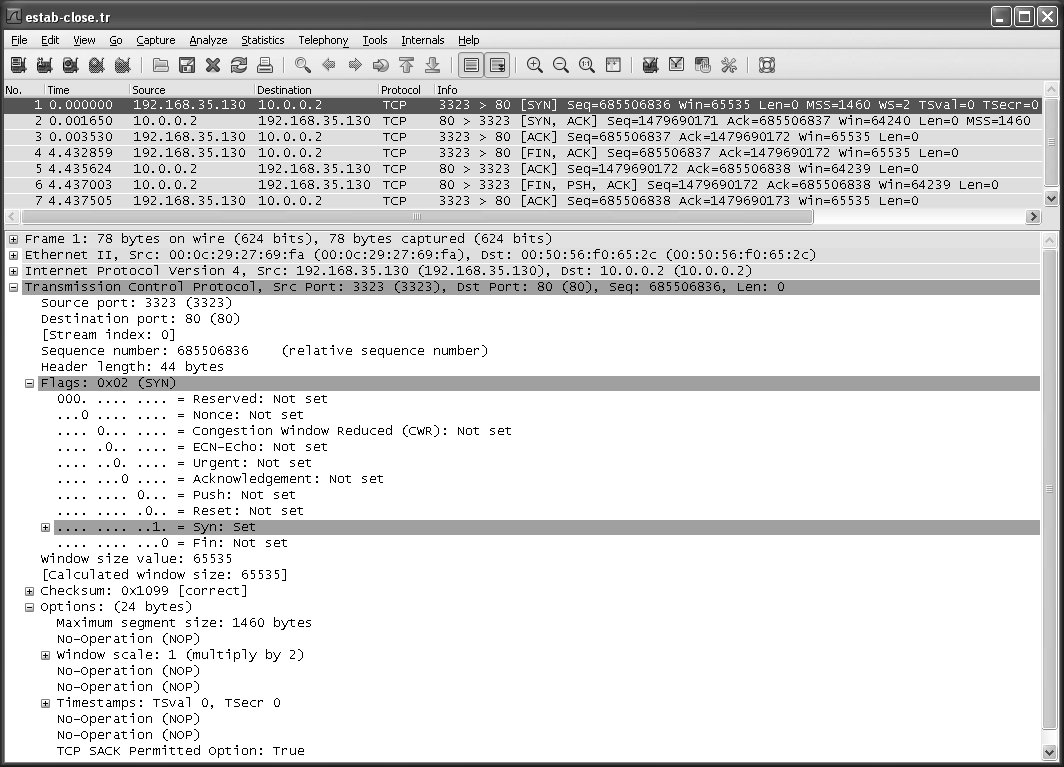
\includegraphics[width=1.0\textwidth]{imgs/13/13-5.png}
	\caption{在主机192.168.35.130与10.0.0.2之间建立一条 TCP 连接,并在不发送任何数据的情况下关闭。PSH(推送)位说明第6个报文段正在发送所有来自缓存的数据(而缓存为空)}
\end{figure}

注意 \href{https://www.rfc-editor.org/rfc/rfc1025}{[RFC1025]} 将拥有最多特性(例如标记与选项)的报文段称力“神风”(kamikaze)数据包。其他生动的术语还包括“丑恶报文”、“圣诞树数据包”、“灯测试”报文段。

从图13-5中我们还会发现SYN报文段包含了一个或多个选项。这些选项需要占用 TCP头部额外的空间。例如,第一个 TCP 头部的长度为44字节,比最小的长度长24字节。TCP
也提供了若干选项,下文将详细介绍当一个连接无法建立时如何使用这些选项。
\subsection{连接建立超时}
本节的若干实例将会展示连接不能建立的情况。一种显而易见的情况是服务器关闭。为了模拟这种情况,我们将 \verb|telnet|命令发送给一个处于同一子网的不存在的主机。在不修改
ARP 表的情况下,上述做法会使客户端收到一个“无法到达主机”的错误消息后退出。由于没有接收到针对之前发送的ARP 请求而返回的ARP 响应(参见第4章),因此会产生“无
法到达主机”的消息。如果我们能事先在 ARP 表中为这个不存在的主机添加一条记录,那么系统就不需要发送 ARP 请求,而会马上根据 TCPAIP 协议尝试与这个不存在的主机建立联
系。相关的命令如下:

\iffalse
	Linux# arp -s 192.168.10.180 00:00:1a: 1b: 10:1đ
	Linux8 date; \verb|telnet| 192.168.10.180 80; date
	7 21:16:34 PDT 2009
	Trying 192.168.10.180...
	to address 192.168.10.180:
	Connection timed out
	7 21:19:43 PDT 2009
\fi

上述例子选择的 MAC地址 00:00:1a:1b:1c:1d 不能与局域网中其他主机的MAC冲突,除此之外并无特别。超时发生在发送初始命令后的3.2分钟。由于没有主机响应,例子中所
有的报文段都是由客户端产生的。清单 13-1 显示了使用 \verb|Wireshark| 软件在摘要模式下获得的输出结果。

有趣的是这些输出结果显示了客户端 TCP 为了建立连接频繁地发送 SYN 报文段。在首个报文段发送后仅3秒第二个报文段就被发送出去,第三个报文段则是这之后的6秒,而第
四个报文段则在第三个报文段发送12秒以后被发送出去,以此类推。这一行为被称作指数回退。在讨论以太网CSMA/CD 介质访问控制协议时(参见第3章)我们也曾见过这样的行
为。然而,这两种指数回退也略有不同。此处的每一次回退数值都是前一次数值的两倍,而在以太网中最大的回退数值是上一次的两倍,实际的回退数值则需要随机选取。

一些系统可以配置发送初始SYN 的次数,但通常选择一个相对较小的数值5。在Linux系统中,系统配置变量 \verb|net.ipv4.tcp_syn_retries| 表示了在一次主动打开申请中尝试重新发送
SYN 报文段的最大次数。相应地,变量\verb|net.ipv4.tcp_synack_retries| 表示在响应对方的一个主动打开请求时尝试重新发送SYN+ACK报文段的最大次数。此外,它能够在设定Linux专
有的TCP\_SYNCNT套接字选项的基础上用于个人连接。正如上面所介绍的,默认的数值为重试5次。两次重新传输之间的指数回退时间是 TCP拥塞管理响应的一部分。当我们讨论
Kam 算法时再仔细研究。
\subsection{连接与转换器}
在第7章,我们已经讨论了一些协议(比如 TCP 和 UDP)如何利用传统的NAT 转换地址与端口号。我们还讨论了 IP 数据包如何在IPv6 与IPv4 两个版本间进行转换。当TCP使
用NAT时,伪头部的校验和通常需要调整(使用校验和中立地址修改器的情况除外)。其他协议也使用伪头部校验和,因为计算包含了与传输层、网络层相关的信息。

当一个 TCP连接首次被建立时,NAT 能够根据报文段的SYN位探明这一事实。同样可以通过检查SYN+ACK报文段与ACK报文段所包含的序列号来判断一个连接是否已经
完全建立。上述方法还适用于连接的终止。通过在 NAT 中实现一部分TCP 状态机(参5IRFC6146]的3.5.2.1 节与3.5.2.2 节)能够跟踪连接,包括当前状态、各方向的序列号以及
相关的 ACK 号。这种状态跟踪是典型的 NAT 实现方法。

当NAT 扮演编辑者的角色并且向传输协议的数据负载中写人内容时,就会涉及一些更复杂的问题。对于 TCP 而言,它将会包括在数据流中添加与删除数据,并由此影响序列号
(与报文段)的长度。此举会影响到校验和,但也会影响数据的顺序。如果利用NAT在数找流中插人或删除数据,这些数值都要做出适当调整。如果 NAT 的状态与终端主机的状态不
同步,连接就无法正确进行下去。因此,上述做法会带来一定的脆弱性。

\section{TCP选项} \label{tcpOpt}
如图12-3所示,TCP 头部包含了多个选项。选项列表结束(End of Option List, EOL)无操作(No Operation, NOP)以及最大段大小(Maximum Segment Size, MSS)是定义于原
始TCP规范中的选项。自那时起,又有若干选项被定义。整个选项列表是由互联网编号分配机构(IANA)维护的[TPARAMS]。表13-1列举了一些目前有趣的选项(即,符合RFC
标准化描述的选项)。

\iffalse
	0

	EOL
	\href{https://www.rfc-editor.org/rfc/rfc0793}{[RFC0793]}
	选项列表结束


	NOP
	(RFC0793]
	无操作(用于填充)


	MSS
	\href{https://www.rfc-editor.org/rfc/rfc0793}{[RFC0793]}
	最大段大小


	WSOPT
	\href{https://www.rfc-editor.org/rfc/rfc01323}{[RFC01323]}
	窗口缩放因子(窗口左移量)


	SACK-Permitted
	\href{https://www.rfc-editor.org/rfc/rfc02018}{[RFC02018]}
	发送者支持 SACK 选项

	可变
	SACK
	\href{https://www.rfc-editor.org/rfc/rfc02018}{[RFC02018]}
	SACK 阻塞(接收到乱序数据)

	10
	TSOPT
	\href{https://www.rfc-editor.org/rfc/rfc01323}{[RFC01323]}
	时间戳选项
	28
	4
	UTO
	\href{https://www.rfc-editor.org/rfc/rfc05482}{[RFC05482]}
	用户超时(一段空闲时间后的终止)
	29
	可变
	TCP-AO
	[RFCO5925]
	认证选项(使用多种算法)
	253
	可变
	Experimental
	\href{https://www.rfc-editor.org/rfc/rfc04727}{[RFC04727]}
	保留供实验所用
	254
	可变
	Experimental
		\href{https://www.rfc-editor.org/rfc/rfc04727}{[RFC04727]}
	保留供实验所用
\fi

每一个选项的头一个字节为“种类”(kind),指明了该选项的类型。根据\href{https://www.rfc-editor.org/rfc/rfc1122}{[RFC1122]},不能被理解的选项会被简单地忽略掉。种类值为0或1的选项仅占用一个字节。其他的选项会
根据种类来确定自身的字节数len。选项的总长度包括了种类与len 个字节。设置 NOP 选项的目的是允许发送者在必要的时候用多个4字节组填充某个字段。需要记住的是 TCP 头部
的长度应该是32比特的倍数,因为TCP 头部长度字段是以此为单位的。EOL 指出了选项列表的结尾,说明无需对选项列表再进行处理。在下文中,我们将详细地探究其他选项。

\subsection{最大段大小选项}
最大段大小是指 TCP 协议所允许的从对方接收到的最大报文段,因此这也是通信对方在发送数据时能够使用的最大报文段。根据[RFCO879],最大段大小只记录 TCP 数据的字
节数而不包括其他相关的TCP 与IP头部。当建立一条TCP 连接时,通信的每一方都要在SYN报文段的MSS 选项中说明自己允许的最大段大小。这16位的选项能够说明最大段大
小的数值。在没有事先指明的情况下,最大段大小的歌认数位为596字节。前文留介绍过,任何主机都应该能够处理至少576字节的IPv4数据报。如果按照最小的 IPv4 与 TCP头
部计算,TCP 协议要求在每次发送时的最大段大小为536字节,这样就正好能够组成一个$576(20+20+536= 576)$字节的IPv4数据报。

图13-5中,最大段大小的数值均为1460。这是IPv4 协议中的典型值,因此IPv4数据数据报的大小也相应增加 40 个字节(总共1500字节,以太网中最大传输单元与互联网路径最大
传输单元的典型数值):20字节的 TCP 头部加20字节的IP 头部。当使用 IPv6协议时,最大段大小通常为1440字节。由于IPv6 的头部比IPv4多20个字节,因此最大段大小的数值相
应减少20字节。在\href{https://www.rfc-editor.org/rfc/rfc2675}{[RFC2675]} 中65535 是一个特数值,与IPv6 超长数据报一起用来指定一个表示无限大的有效最大段大小值。在这种情况下,发送方的最大段大小等于路径MTU
的数值减去60字节(40字节用于IPv6头部,20字节用于 TCP 头部)。值得注意的是,最大段大小并不是TCP 通信双方的协商结果,而是一个限定的数值。当通信的一方将自己的最
大段大小选项发送给对方时,它已表明自己不愿意在整个连接过程中接收任何大于该尺寸的报文段。

\subsection{选择确认选项}
第12 章介绍了滑动窗口的概念,并描述了TCP 协议是如何管理序列号与确认的。由于采用累积 ACK确认,TCP不能正确地确认之前已经接收的数据。由于接收的数据是无序的,
所以接收到数据的序列号也是不连续的。在这种情况下,TCP 接收方的数据队列中会出现空洞的情况。因此在提供字节流传输服务时,TCP接收方需要防止应用程序使用超出空洞的
数据。

如果 TCP 发送方能够了解接收方当前的空洞(以及在序列空间中超出空洞的乱序数据块),它就能在报文段丢失或被接收方遗漏时更好地进行重传工作。根据\href{https://www.rfc-editor.org/rfc/rfc2018}{[RFC2018]}与
\href{https://www.rfc-editor.org/rfc/rfc2883}{[RFC2883]},TCP“选择确认”(SACK)选项提供了上述功能。如果 TCP接收方能够提供选择确认信息,并且发送方能够合理有效地利用这些信息,那么上述方案将会十分高效。

通过接收SYN(或者 SYN +ACK)报文段中的“允许选择确认”选项,TCP通信方会了解到自身具有了发布SACK 信息的能力。当接收到乱序的数据时,它就能提供一个 SACK
选项来描述这些乱序的数据,从而帮助对方有效地进行重传。SACK 信息保存于SACK 选项中,包含了接收方已经成功接收的数据块的序列号范围。每一个范围被称作一个SACK块,
由一对32 位的序列号表示。因此,一个 SACK 选项包含了n个 SACK块,长度为(8n +2)个字节。增加的2个字节用于保存SACK 选项的种类与长度。

由于TCP 头部选项的空间是有限的,因此一个报文段中发送的最大SACK 块数目为3(假设使用了时间戳选项。根据13.3.4节的介绍,这是现代 TCP 实现中的典型情况)。虽然只
有SYN报文段才能包含“允许选择确认”选项,但是只要发送方已经发送了该选项,SACK块就能够通过任何报文段发送出去。由于选择确认的操作相对于 TCP的错误和拥塞控制的
操作而言更简单,本书将在第14 章与第16章再介绍相关的细节。
\subsection{窗口缩放选项}
根据 \href{https://www.rfc-editor.org/rfc/rfc1323}{[RFC1323]},窗口缩放选项(表示 WSCALE 或 WSOPT) 能够有效地将 TCP 窗口广告字段的范围从16 位增加至30位。TCP 头部不需要改变窗口通告字段的大小,仍然维持
16位的数值。同时,使用另一个选项作为这16位数值的比例因子。该比例因子能够使窗口字段值有效地左移。这样事实上将窗口数值 大至原先的$2^n$倍,其中$n$为比例因子。一个字
节的移动可以用0至14(包含14)来计数。计数。的移动表示没有任何比例。最大的比例数值是14,它能够提供一个最大为1 073 725440字节$(65535 ×2^(14))$的窗口。该数值接
近$1073 741 823(2^(30)-1)$,正好1GB。因此,TCP使用一个32位的值来维护这个“真实”的窗口大小。

该选项只能出现于一个SYN报文段中,因此当连接建立以后比例因子是与方向绑定的。为了保证窗口调整,通信双方都需要在SYN报文段中包含该选项。主动打开连接的一方利
用自己的SYN中发送该选项,但被动打开连接的一方只能在接收到的SYN 中指出该选项时才能发送。每个方向的比例因子可各不相同。如果主动打开连接的一方发送了一个非0的比
例因子但却没有接收到来自对方的窗口缩放选项,它会将自己发送与接收的比例因子数值都设为0。这样使得系统不需要理解这些系统间的选项互操作。

假设我们正在使用窗口缩放选项,发送出去的窗口移动数值S,而接收到的窗口移动数值为R。这样,我们从对方接收到每一个16位的广告窗口都需要左移R位才能获得真实
窗口大小。每次向对方发送窗口通告时,都会将32位的窗口大小向右移动S位,然后将16位的数值填充到 TCP头部。

窗口的移动数值是由 TCP通信方根据接收缓存的大小自动选取的。缓存的大小是由系统设定的,但是应用程序通常都具有改变其大小的能力。当TCP协议被用于在大带宽、高
延迟网络(即,往返时间与带宽都相对较大的网络)上提供海量数据传输服务时,窗口缩放选项就非常有意义。因此,第16章将会进一步讨论该选项的重要性与使用方法。

\subsection{时间戳选项与防回绕序列号}
时间戳选项(记作 TSOPT 或TSopt)要求发送方在每一个报文段中添加2个4字节的时间戳数值。接收方将会在确认中反映这些数值,允许发送方针对每一个接收到的ACK 估
算 TCP连接的往返时间(由于 TCP 协议经常利用一个ACK 来确认多个报文段,此处必须指出是“每个接收到的ACK”而不是“每个报文段”。本书第15 章将会详细地讨论这一问
题)。当使用时间戳选项时,发送方将一个32位的数值填充到时间戳数值字段(称作 TSV 或TSval)作时间戳选项的第一个部分;而接收方则将收到的时间戳数值原封不动地填充至第
二部分的时间截回显重试字段(称作 TSBR 或 TSecr)。由于包含了时间截选项,TCP 头部的长度将会增长 10字节(8字节用于保存2个时间戳数值,而另2个数值则用于指明选项的数
值与长度)。

时间戳是一个单调增加的数值。由于接收者只会对它接收到的信息做出响应,所以它并不关心时间戳单元或数值到底是什么。该选项并不要求在两台主机之间进行任何形式的时钟
同步。\href{https://www.rfc-editor.org/rfc/rfc1323}{[RFC1323]} 推荐发送者每秒钟至少将时间戳数值加1。图13-6显示了通过 Wireshark软件获得的时间戳选项。

上述例子中,通信双方都产生并回应了对方的时间戳。第一个报文段(客户端的SYN)使用一三个初始的时间戳数位 81813090。该数值被域充在时间破数位子段中。由于容户端
并不知道服务器的时间戳数值,所以该报文段的第二部分时间戳回显重试字段的数值为0。

一个使用了时间戳、窗口缩放以及最大段大小选项的TCP连接。TCP头部长度为44字节。
初始SYN(第1个数据包)的时间戳数值为81813090。图中高亮标记的第二个数据包将这一数值作为响应返回给主动打开连接的一方,同时包含了自己的数值349742014

估算一条TCP连接的往返时间主要是为了设置重传超时。重传超时用于告知TCP通信方何时应该重新发送可能已经丢失的报文段。第12章已经讨论了在一些往返时间函数
的基础上设置此项超时的必要性。借助时间戳选项,我们能够获得往返时间相对精确的测量结果。在使用时间戳选项之前,大多 TCP通信会针对每个窗口的数据抽取一个往返时间
样本。时间戳选项使我们获得了更多的样本,从而提升了精确估算往返时间的能力(参见[RFC13231 与 \href{https://www.rfc-editor.org/rfc/rfc6298}{[RFC6298]})。

由于时间戳选项与重传计时器的设置紧密相关,我们将在第14 章讨论重传问题时详细地介绍时间戳选项的这一用途。“这一用途”是为了强调虽然时间戳选项允许更高频率的往
返时间样本,但它也为接收者提供了避免接收旧报文段与判断报文段正确性的方法。这被称作防回绕序列号(Protection Against Wrapped Sequence numbers, PAWS),它与时间戳选项
一起记录于\href{https://www.rfc-editor.org/rfc/rfc1323}{[RFC1323]}中。现在,我们要继续探究一下它是如何工作的。

假设一个 TCP 连接使用了窗口缩放选项,并将其设置为可能最大的窗口,大约1GB。再假设使用了时间戳选项,并且发送者针对发送的每个窗口分配的时间戳数值都会加1。(这
一假设是保守的。正常情况下时间戳数值的增长速度要远快于此。)表13-2显示了当传输6GB 数据时两个主机之间可能的数据流。为了避免过多的10位数字,我们使用符号G表
示1073 741824 的倍数。我们还再次采用了 tcpdump 中的符号J:K来表示从第J个字节到第K-1个字节的数据。

TCP时间戳选项通过提供一个额外的32位有效序列号空间清除了具有相同序列号的报文段之间的二义性

32位序列号字段在时刻D和时刻E间回绕。假设在时刻B有一个报文段丢失并被亘传。又假设这一丢失的报文段在时刻F重新出现。假设报文段丢失与重新出现的时间差小于
一个报文段在网络中存在的最大时间(称为 MSL,参见13.5.2节),否则当路由器发现TTL期满后就会丢弃该报文段。正如我们之前提到的,旧的报文段重新出现并包含当前正在传输
的序列号的问题只会发生在相对高速的连接中。

由表13-2可以看出,使用时间戳选项能够有效地防止上述问题。接收者可以将时间言看作一个32位的扩展序列号。丢失的报文段会在时刻F重新出现,由于它的时间戳为2,小
于最近的有效时间戳(5或6),因此防回绕序列号算法会将其丢弃。防回绕序列号算法并不要求在发送者与接收者之间有任何形式的时钟同步。接收者所需要的是保证时间戳数值单调
增长,并且每一个窗口的数据至少增加1。

\subsection{用户超时选项}
根据TRFC5482]的描述,用户超时(UTO)选项是一个相对较新的TCP 的功能。用户超时数值(也被称力 USER\_TIMEOUT) 指明了 TCP 发送者在确认对方未能成功接收数据之前
愿意等待该数据 ACK 确认的时间。根据\href{https://www.rfc-editor.org/rfc/rfc0793}{[RFC0793]},USER\_TIMEOUT 是 TCP 协议本地配置的一个参数。用户超时选项允许TCP 通信方将自己的USER\_TIMEOUT 数值告知连接的
对方。这样就方便了 TCP 接收方调整自己的行为(例如,在终止连接之前容忍一段较长时间的连接中断)。NAT设备也能够解释这些信息以帮助设置它们的连接活动计时器。

用户超时选项的数值是建议性的,因为即便连接的一端希望使用一个大的或小的数信也不意味着另一端就必须遵从。[RFCI122]提炼了 USER\_TINEOUT 的定义,并且建议当
TCP 连接达到3次重传阈值时应该通知应用程序(规则1),而当超时大于100秒时应该关闭连接(规则2)。某些实现会提供 API 函数来修改规则1与规则2。由于长的用户超时设置
会导致资源耗尽,而短的用户超时设置可能会导致一些连接过早地断开(例如,拒绝服务攻击),因此需要为用户超时选项的可能数值设置上下边界。设置 USER\_TIMEOUT 的具体方
法如下:
USER\_TIMEOUT = min(U\_LIMIT, max (ADV\_UTO, REMOTE\_UTO, L\_LIMIT) )

其中 ADV\_UTO 是本端告知远端通信方的用户超时选项数值,而 \_UTO是远端通信方告知的用户超时选项数值,U\_LIMIT 是本地系统对用户超时选项设定的数值上边界
,而L\_LIMIT 则是下边界。值得注意的是上式并不能保证同一连接的两端会获得相同的用户超时数值。在任何情况下,L\_LIMIT 的数值必须大于对应连接的重传超时数值(参见第1
章)。L\_LINIT的数值一般推荐设为100 秒,这样可以保持与『RFC1122]相兼容。

建立连接的 SYN报文段、首个非SYN报文段以及 USER\_TIMEOUT 的数值发生任何改变的报文段,都会包含用户超时选项。该选项的数值由一个 15位的数值部分与一个1位的
单位部分构成。单位部分用于说明数值的计量单位是分钟(1)还是秒(0)。UTO 作为一个相对较新的选项还没有得到广泛使用。

\subsection{认证选项}
TCP设置了一个选项用于增强连接的安全性。设计该选项的目的在于增强与替换较早的TCP-MDS 机制 \href{https://www.rfc-editor.org/rfc/rfc2385}{[RFC2385]}。这一选项被称作TCP 认证选项 (TCP Authentication Option,
TCP-AO)\href{https://www.rfc-editor.org/rfc/rfc5925}{[RFC5925]},它使用了一种加密散列算法(参见第18章)以及 TCP连接双方共同维护的一个秘密值来认证每一个报文段。TCP 认证选项不仅提供各种加密算法,还使用“带
内”信令来确认密钥是否改变,因此它与TCP-MDS 相比有很大的提高。然而,TCP 认证选项没有提供一个全面密钥管理方案。也就是说,通信双方不得不采用一种方法在TCP认证
选项运行之前建立出一套共享密钥。

当发送数据时,TCP 会根据共享的密钥生成一个通信密钥,并根据一个特的加密算法[RFCS926] 计算散列值。接收者装配有相同的密钥,同样也能够生成通信密钥。借助通信密
钥,接收者可以确认到达的报文段是否在传输过程中被篡改过(有非常高的可能性)。设置该选项是为了针对各种 TCP 欺骗攻击提供强有力的抵御策略(参见13.8节)。然而,由于需
要创建并分发一个共享密钥(这是一个相对新的选项),该选项并没有得到广泛使用。
\section{TCP 的路径最大传输单元发现}
第3章介绍了路径最大传输单元(MTU)的概念。它是指经过两台主机之间路径的所有网络报文段中最大传输单元的最小值。知道路径最大传输单元后能够有助于一些协议(比如
TCP)避免分片。第10章介绍了基于ICMP消息的路径最大传输单元发现(PMTUD)过程是如何实现的,但由于应用程序已经指定了尺寸(即,非传输层协议),UDP协议一般不会
采用上述发现过程获得的数据报大小。TCP 在支持字节流抽象的实现过程中能够决定使用多大的报文段,因此它很大程度上控制了最后生成的IP数据包。

在本节中,我们将会进一步探寻 TCP 是如何使用路径最大传输单元的。我们的讨论内容适用于 TCP/IPv4 与TCP/IPV6。\href{https://www.rfc-editor.org/rfc/rfc1191}{[RFC1191]}与\href{https://www.rfc-editor.org/rfc/rfc1981}{[RFC1981]}能分别提供更多的细节。一种称
作分组层路径最大传输单元发现(Packetization Layer Path MTU Discovery, PLPMTUD)的算法能够避免对ICMP的使用。根据\href{https://www.rfc-editor.org/rfc/rfc4821}{[RFC4821]},该算法也能够被TCP或其他传输协议使
用。我们可以利用 IPv6 协议中 “数据包太大”(Packet Too Big, PTB)的术语来代表 ICMIPv4地址不可达(需要分片)或ICMPv6 数据包太大的消息。

TCP 常规的路径最大传输单元发现过程如下:在一个连接建立时,TCP 使用对外接口的最大传输单元的最小值,或者根据通信对方声明的最大段大小来选择发送方的最大段大小
(SMSS)。路径最大传输单元发现不允许 TCP 发送方有超过另一方所声明的最大段大小的行为。如果对方没有指明最大段大小的数值,发送方将假设采用默认的536字节,但是这种情
况比较少见。如果为每一个目的地保存对应的路径最大传输单元,那么就能方便地对段大小进行选择。值得注意的是,一条连接的两个方向的路径最大传输单元是不同的。

一旦为发送方的最大大小选定了初始值,TCP通过这条连接发送的所有IPv4 数据报都会对 DF位字段进行设置。TCP/IPv6 没有DF 位字段,因此只需要假设所有的数据报都已经
设置了该字段而不必进行实际操作。如果接收到 PTB 消息,TCP 就会减少段的大小,然后用修改过的段大小进行重传。如果在PTB 消息中已包含了下一眺推荐的最大传输单元,段
大小的数值可以设置为下一眺最大传输单元的数值减去 IPv4(或IPv6)与TCP头部的大小。如果下一眺最大传输单元的数值不存在(例如,一个之前的ICMP 错误被返回时会缺乏这一
信息),发现者可能需要尝试多个数值(例如,采用二分搜案法选择一个可用的数值)。这也会影响到 TCP的拥塞控制管理(参见第16 章)。对于分组层路径最大传输单元发现而言,除
了PTB的消息不被使用以外其他情况基本类似。相反,执行路径最大传输单元发现的协议必须能够快速地检测消息丢弃并调整自己的数据报大小。

由于路由是动态变化的,在减少段大小的数值一段时间后需要尝试一个更大的数值(接近初始的发送方最大段大小)。根据\href{https://www.rfc-editor.org/rfc/rfc1191}{[RFC1191]}与\href{https://www.rfc-editor.org/rfc/rfc1981}{[RFC1981]}的指导意见,该时间间隔大约
为10分钟。

在互联网环境中,由于防火墙阻塞 PTB 消息\href{https://www.rfc-editor.org/rfc/rfc2923}{[RFC2923]},路径最大传输单元发现过程会存在一些问题。在各种操作问题中,黑洞问题的情况虽有所好转(在[LS10]中,80\%被调查
的系统都能够正确地处理PTB 消息),但仍悬而未决。在 TCP 实现依靠传输 ICMP 消息来调整它的段大小的情况下,如果 TCP 从未接收到任何ICMP 消息,那么在路径最大传输单元发
现过程中就会造成黑洞问题。这种情况可能由多方面的原因造成,其中包括了防火墙或NAT配置为禁止转发ICMP 消息。其后果在于一旦 TCP使用了更大的数据包将不能被正确处理。
由于只是不能转发大数据包,所以诊断出这一问题是十分困难的。那些较小的数据包(比如用于建立连接的 SYN与SYN +ACK 数据包)是能够成功处理的。一些TCP 实现具有“黑
洞探测”功能。当一个报文段在反复重传数次后,将会尝试发送一个较小的报文段。
\subsection{例子}
当中间路由器的最大传输单元小于任何一个通信端的最大段大小时,TCP 就会执行路径最大传输单元发现过程。为了创造上述条件,本文使用一台路由器(一台本地地址为
\verb|10.0.0.1| 的Linux 主机)通过PPPoE 接口连接DSL 服务提供商。PPPoE 链路使用的最大传输单元为1492字节(以太网的最大传输单元为1500字节,减去 PPPOE协议的6字节负载,再
减去2字节的 PPP 负载。参见第13章)。图13-7显示了上述例子的拓扑结构。

PPPoE 封装使 TCP 连接的路径最大传输单元从1500字节(以太网最大传输单元的典型值)减至
1492字节。为了证明 TCP的路径 MTU 发现功能,此例设置了更小的最大传输单元(288予节)

为了更加明显地看出这一行为,将 PPPOE 链路最大传输单元的数值以1492减少至288字节。通过在图13-7的GW 主机上执行下面的命令来完成这项工作:

此外,还需要告知客户端(图13-7中的c)系统允许的最小报文段大小:

如果不执行第2步操作,Linux 系统会将路径最大传输单元的最小值设置为默认的552字节,这样就能够避免某些较小的最大传输单元攻击(参见13.8节)。这样做的后果是此例
中任何大于288字节的数据包都将被分片。为了避免这种情况的发生,并证明路径最大传输单元发现是有效的,需要修改这一最小值。然后,我们开始通过互联网从主机C(地址
\verb|10.0.0.1|23)向服务器S传输文件(地址 169.229.62.97)。清单13-2显示了利用 tcpdump记录下的数据包交换过程。为了清楚起见,隐藏了一些行并删除了一些不相关的字段。

在网络传输过程中,如果中间链路的最大传输单元小于两端通信节点的,路径MTU 发现机制能够找出合适的段大小以供传输使用

根据 tcpdump 的输出结果,连接已经建立并且最大段大小的数值已经交换。连接中所有的数据包都将 DF 位置位,所以两端都能够使用路径 MTU 发现机制。较远一方的首个数据
包的长度为588字节。尽管中间 PPPoE链路的最大传输单元已配置为288字节,但该数据包仍能够成功地通过路由器转发而不被分片。产生这种情况的原因是不对称的最大传输单元
配置。虽然 PPPoE 链路的本地端使用了288字节的最大传输单元,但是另一端仍然将发送方最大段大小的数值设置为一个较大的值,大概是1492字节。这样就会造成下述情况,向
外发送的数据包需要较小的段大小(288字节或更小),而反方向进入的数据包可以拥有较大的段大小。

当本地通信端尝试发送一个588字节且 DF 位置位的较大数据包时,路由器(\verb|10.0.0.1|)将会产生一个PTB 消息,指出适合下一跳链路的最大传输单元大小为288字节。在收到这
条PTB消息后,TCP 在发送下一个数据包时会按照指示选择288字节作为响应。对于那些原本打算以588字节的大小发送的剩余的数据包,TCP也会按照最大传输单元的数值将它们
重新划分,另外发送两个大小分别为288 字节与116 字节的数据包。在文件传输的过程中,类似的数据包大小会不断地重复出现。

路径 MTU 发现过程是一种 TCP 明确地尝试调整段大小的方法。它适用于 TCP 连接建立后,至少是在传输大量数据时。报文段的大小能够影响吞吐量的总体性能以及 TCP 窗口
大小。第15 章将会继续讨论它是如何影响总体性能的。
\section{TCP 状态转换}
我们已经介绍了许多关于一个 TCP 连接启动与终止的规则,也看到了在一个连接的不同阶段需要发送的各种类型的报文段。这些决定 TOP 应该做什么的规则其实是由 TCP 所属的状
态决定的。当前的状态会在各种触发条件下发生改变,例如传输或接收到的报文段、计时器超时、应用程序的读写操作,以及来自其他层的信息。这些规则可以概括为 TCP 的状态转换图。

\subsection{TCP 状态转换图}
图13-8展示了 TCP 的状态转换图。图中的状态用椭圆表示,而状态之间的转换则用箭头表示。TCP连接的每一端都可以在这些状态中进行转换。有些转换是由于接收到某个控制
位字段置位的报文段而引发的(例如,SYN,ACK,FIN);而有些转换又会要求发送一些控制位字段置位的报文段。另外还有一些转换是由应用程序的动作或计时器超时引发的。上述
各种情况都以文本注释的方式标记在转换图的相关箭头旁边。当初始化时,TCP 从 CLOSED状态启动。通常根据是执行主动打开操作还是被动打开操作,TCP 将分别快速转换到SYN\_
SENT 或LISTEN 状态。

TCP 状态转换图(也称作有限状态机)。箭头表示因报文段传输、接收以及计时器超时而引发的状态转换。粗箭头表示典型的客户端的行为,虚线箭头表示典型的服务器行为。粗体指令
(例如 open、close)是应用程序执行的操作

图13-8中值得注意的是只有一部分状态转移被认为是“典型的”。我们已经将普通的客户端状态转移用深黑的实线箭头表示,而普通的服务器状态转换用虚线箭头表示。导向
ESTABLISHED 状态的两种转换与打开一个连接相关,从ESTABLISHED 状态导出的两种转换则用于终止一个连接。ESTABLISHED 是通信双方双向传输数据的状态。第14~17章将
详细地介绍该状态。

\begin{center}
	\begin{tikzpicture}[>=latex]

		%
		% Styles for states, and state edges
		%
		\tikzstyle{state} = [draw, very thick, fill=white, rectangle, minimum height=3em, minimum width=7em, node distance=8em, font={\sffamily\bfseries}]
		\tikzstyle{stateEdgePortion} = [black,thick];
		\tikzstyle{stateEdge} = [stateEdgePortion,->];
		\tikzstyle{edgeLabel} = [pos=0.5, text centered, font={\sffamily\small}];

		%
		% Position States
		%
		\node[state, name=closedStart] {CLOSED};
		\node[state, name=listen, below of=closedStart] {LISTEN};
		\node[state, name=synSent, below of=listen, right of=listen, xshift=8em] {SYN\_SENT};
		\node[state, name=synRcvd, below of=listen, left of=listen, xshift=-8em] {SYN\_RCVD};
		\node[state, name=established, below of=listen, node distance=14em] {ESTABLISHED};
		\node[state, name=finWait1, below of=established, left of=established, node distance=7em, xshift=-9em] {FIN\_WAIT\_1};
		\node[state, name=finWait2, below of=finWait1] {FIN\_WAIT\_2};
		\node[state, name=closeWait, below of=established, right of=established, node distance=7em, xshift=9em] {CLOSE\_WAIT};
		\node[state, name=closing, below of=established, node distance=14em] {CLOSING};
		\node[state, name=lastAck, below of=closeWait] {LAST\_ACK};
		\node[state, name=timeWait, below of=closing] {TIME\_WAIT};

		%
		% Connect States via edges
		%
		\draw ($(closedStart.south) + (-.5em,0)$)
		edge[stateEdge] node[edgeLabel, xshift=-3em]{\emph{Passive open}}
		($(listen.north) + (-.5em,0)$);
		\draw ($(listen.north) + (.5em,0)$)
		edge[stateEdge] node[edgeLabel, xshift=2em]{\emph{Close}}
		($(closedStart.south) + (.5em,0)$);

		\draw ($(listen.south) + (-1em,0)$)
		edge[stateEdge, bend left=22.5] node[edgeLabel, xshift=-2em, yshift=1em]{SYN/SYN + ACK}
		($(synRcvd.east) + (0,1em)$);
		\draw ($(listen.south) + (1em,0)$)
		edge[stateEdge, bend right=22.5] node[edgeLabel, xshift=1em, yshift=1em]{\emph{Send}/SYN}
		($(synSent.west) + (0,1em)$);

		\draw ($(synRcvd.north) + (.5em,0)$)
		edge[stateEdge, bend left=45] node[edgeLabel,xshift=-4em]{\emph{Timeout}/RST}
		($(closedStart.west) + (0,-.5em)$);

		\draw ($(synSent.north) + (-.5em,0)$)
		edge[stateEdge, bend right=45] node[edgeLabel,xshift=-1em, yshift=-1em]{\emph{Close}}
		($(closedStart.east) + (0,-.5em)$);
		\draw ($(closedStart.east) + (0,.5em)$)
		edge[stateEdge, bend left=45] node[edgeLabel,xshift=4em]{\emph{Active open}/SYN}
		($(synSent.north) + (.5em,0)$);

		\draw (synSent.west)
		edge[stateEdge] node[edgeLabel, yshift=1em]{SYN/SYN + ACK}
		(synRcvd.east);
		\draw (synRcvd)
		edge[stateEdge] node[edgeLabel, xshift=-2.5em]{\emph{Close}/FIN}
		(finWait1);

		\draw ($(synRcvd.east) + (0,-1em)$)
		edge[stateEdge, bend left=22.5] node[edgeLabel, xshift=-1em, yshift=-1em]{ACK}
		($(established.north) + (-1em,0)$);
		\draw ($(synSent.west) + (0,-1em)$)
		edge[stateEdge, bend right=22.5] node[edgeLabel, xshift=3em, yshift=-1em]{SYN + ACK/ACK}
		($(established.north) + (1em,0)$);

		\draw ($(established.south) + (-1em,0)$)
		edge[stateEdge, bend left=22.5] node[edgeLabel, xshift=-1em, yshift=1em]{\emph{Close}/FIN}
		($(finWait1.east) + (0,.5em)$);
		\draw ($(established.south) + (1em,0)$)
		edge[stateEdge, bend right=22.5] node[edgeLabel, xshift=1em, yshift=1em]{FIN/ACK}
		($(closeWait.west) + (0,1em)$);

		\draw (finWait1.south)
		edge[stateEdge] node[edgeLabel, xshift=-2em]{ACK}
		(finWait2.north);
		\draw ($(finWait1.east) + (0,-.5em)$)
		edge[stateEdge, bend left=22.5] node[edgeLabel, yshift=1em]{ACK}
		(closing.north);
		\draw (finWait1.south east)
		edge[stateEdge] node[edgeLabel, xshift=1em, yshift=2em, text width=3em]{FIN + ACK/ACK}
		(timeWait.north west);

		\draw (finWait2.south)
		edge[stateEdge, bend right=22.5] node[edgeLabel, xshift=-2em, yshift=-1em]{FIN/ACK}
		(timeWait.west);

		\draw (closing)
		edge[stateEdge] node[edgeLabel, xshift=-2em]{ACK}
		(timeWait);

		\draw (closeWait)
		edge[stateEdge] node[edgeLabel,xshift=2.5em]{\emph{Close}/FIN}
		(lastAck);

		%
		% Connect lastAck to closed is slightly more complicated
		% no direct line-of-sight, so we need to take the scenic route
		%
		\coordinate (lastAck2ClosedA) at ($(lastAck.east) + (2em,0)$);
		\coordinate (lastAck2ClosedB) at ($(closedStart.north -| lastAck.east) + (2em,1em)$);
		\coordinate (lastAck2ClosedC) at ($(closedStart.north) + (0.5em,1em)$);
		\draw (lastAck.east) edge[stateEdgePortion] (lastAck2ClosedA);
		\draw (lastAck2ClosedA) edge[stateEdgePortion] node[edgeLabel,xshift=-1.5em, yshift=-4em]{ACK} (lastAck2ClosedB);
		\draw (lastAck2ClosedB) edge[stateEdgePortion] (lastAck2ClosedC);
		\draw (lastAck2ClosedC) edge[stateEdge] ($(closedStart.north) + (0.5em,0)$);

		%
		% likewise for timeWait to closed
		%
		\coordinate (timeWait2ClosedA) at ($(timeWait.south) + (0,-1em)$);
		\coordinate (timeWait2ClosedB) at ($(timeWait.south -| finWait2.west) + (-2em,-1em)$);
		\coordinate (timeWait2ClosedC) at ($(closedStart.north -| finWait2.west) + (-2em,1em)$);
		\coordinate (timeWait2ClosedD) at ($(closedStart.north) + (-0.5em,1em)$);
		\draw (timeWait.south) edge[stateEdgePortion] (timeWait2ClosedA);
		\draw (timeWait2ClosedA) edge[stateEdgePortion] (timeWait2ClosedB);
		\draw (timeWait2ClosedB) edge[stateEdgePortion] (timeWait2ClosedC);
		\draw (timeWait2ClosedC) edge[stateEdgePortion]
		node[edgeLabel, text width=12.25em, yshift=1.5em]{\emph{Timeout after two maximum segment lifetimes (2*MSL)}}
		(timeWait2ClosedD);
		\draw (timeWait2ClosedD) edge[stateEdge] ($(closedStart.north) + (-0.5em,0)$);

		% draw dotted lines around passive and active closes
		\begin{pgfonlayer}{background}
			\draw [join=round,black,dotted] ($(closeWait.north west) + (-1em, -1em)$) rectangle ($(lastAck.south east) + (1em, 1em)$);
			\draw [join=round,black,dotted] ($(finWait1.north west) + (-1em, -1em)$) rectangle ($(timeWait.south east) + (1em, 1em)$);
		\end{pgfonlayer}

	\end{tikzpicture}
\end{center}

图 13-8将FIN\_WAIT\_I、FIN\_WAIT\_2 以及 \verb|TIME_WAIT| 状态用一个方框括起来(至少是部分被括起来),称作“主动关闭”。它们表示当本地应用程序发起一个关闭请求时会进入
的状态集合。另外两个状态(CLOSE\_WAIT 与LAST\_ACK)被一个虚线框括起来,并标记为“被动关闭”。这些状态与等待一个节点确认一个 FIN 报文段并进行关闭相关。同时关闭
可以视为一种包含两个主动关闭的形式。此外,还使用了CLOSING状态。

图13-8中的11种状态名称(CLOSED、LISTEN、SYN\_SENT等)都是基于 UNIX、Linux、Windows 系统中 netstat命令所输出的名称。而这些名称则是参考了\href{https://www.rfc-editor.org/rfc/rfc0793}{[RFC0793]}中的
名称。CLOSED 状态并不能算作一个“官方”的状态,但在图13-8 中却被作为一个开始状态点和一个终止状态点。

从LISTEN 到 SYN\_SENT 的状态转换在TCP 协议中是合法的,但却不被伯克利套接字所支持,因此比较少见。从SYN\_RCVD返回到 LISTEN 的状态转换只有在 SYN\_RCVD状
态是由LISTEN 状态(在正常的场景中)而非 SYN\_SENT 状态转换而来的情况下才是正确的。这意味着,如果我们执行一个被动打开操作(进入LISTEN 状态),接收一个SYN,发
送一个带有ACK 确认的SYN(进入SYN\_RCVD状态),然后收到一个重置消息而非ACK,端点就会返回到 LISTEN 状态,并且等待另一个连接请求的到来。

图13-9不仅显示了正常TCP连接的建立与终止过程,还详细介绍了客户端与服务器经历的各种状态。它是图13-1 的简略版本,在显示相关状态的同时省略了选项与初始序列号
等细节。假设在图 13-9中左侧的客户端执行一个主动打开操作,而右侧的服务器执行一个被动打开操作。虽然根据前文的介绍由客户端负责执行主动关闭操作,但是通信的任何一方
都能够进行这项工作。

\subsection{ TIME\_WAIT 状态 }
\verb|TIME_WAIT|状态也称为2MSL等待状态。在该状态中,TCP 将会等待两倍于最大段生存期(Maximum Segment Lifetime, MSL)的时间,有时也被称作加倍等待。每个实现
都必须为最大段生存期选择一个数值。它代表任何报文段在被丢弃前在网络中被允许存在的最长时间。我们知道这个时限是有限制的,因为TCP 报文段是以IP数据报的形式传输的,IP数
据报拥有 TTL 字段和跳数限制字段。这两个字段限制了 IP 数据报的有效生存时间(参见第5章)。\href{https://www.rfc-editor.org/rfc/rfc0793}{[RFC0793]} 将最大段生存期设为2分钟。然而在常见实现中,最大段生存期的数值可
以为30秒、1分钟或者2分钟。在绝大多数情况下,这一数值是可以修改的。在Linux 系统中,\verb|net.ipv4.tcp_fin_timeout| 的数值记录了 2MSL 状态需要等待的超时时间(以秒为单位)。
在 Windows 系统,下面的注册键值也保存了超时时间:
\begin{lstlisting}[language=bash]
HKLM\SYSTEM\CurrentControlSet\Services\Tcpip\Parameters\TcpTimedWaitDelay
\end{lstlisting}
该键值的取值范围是30~300秒。对于 IPv6 而言,只需要将键值中的Topip 替换为 Topip6即可。

假设已设定 MSL 的数值,按照规则:当TCP执行一个主动关闭并发送最终的ACK 时,连接必须处于 \verb|TIME_WAIT| 状态并持续两倍于最大生存期的时间。这样就能够让 TCP 重新
发送最终的ACK以避免出现丢失的情况。重新发送最终的ACK 并不是因为TCP 重传了ACK(它们并不消耗序列号,也不会被TCP重传),而是因为通信另一方重传了它的FIN(它
消耗一个序列号)。事实上,TCP 总是重传 FIN,直到它收到一个最终的ACK。

另一个影响2MSL 等待状态的因素是当TCP 处于等待状态时,通信双方将该连接(客户端卫地址、客户端端口号、服务器I地址、服务器端口号)定义为不可重新使用。只有
当2MSL 等待结束时,或一条新连接使用的初始序列号超过了连接之前的实例所使用的最高序列号时\href{https://www.rfc-editor.org/rfc/rfc1122}{[RFC1122]},或者允许使用时间戳选项来区分之前连接实例的报文段以避免混淆时
IRFC619]],这条连接才能被再次使用。不幸的是,一些实现施加了更加严格的约束。在这些系统中,如果一个端口号被处于 2MSL 等待状态的任何通信端所用,那么该端口号将不能
被再次使用。清单 13-3与清单13-4展示了这一约束的相关例子。

许多实现与API都提供了绕开这一约束的方法。在伯克利套接字API 中,SO\_RBUSEADDR 套接字选项就支持绕开操作。它允许调用者为自己分配本地端口号,即使这个
端口号是某个处于2MSL 等待状态连接的一部分。我们还会发现,即使套接字(地址、端口号对)具有绕开机制,TCP的规则仍会防止该端口号被处于 2MSL等待状态的同一连接的其
他实例重新使用。当一个连接处于 2MSL 等待状态时,任何延迟到达的报文段都将被丢弃。因为一条连接是通过地址和端口号的4元组定义的。如果该连接处于 2MSL 等待状态,那么
它在这段时间内将不能被重新使用。当这条正确的连接最终被建立起来后,这条连接之前的实例所传输的延迟报文段是不能被当作新连接的一部分来解读的。

对于交互式应用程序而言,客户端通常执行主动关闭操作并进入 \verb|TIME_WAIT| 状态,服务器通常执行被动关闭操作并且不会直接进入\verb|TIME_WAIT|状态。其中的含义是,如果我们
终止一个客户端后立刻重新启动同一客户端,那么新的客户端也不能重新使用相同的本地端口号。通常来说,这并不成问题。因为客户端通常使用的是由操作系统分配的临时端口号,
而且它们也并不关心被分配的端口号究竞是什么(回忆一下,实际上出于安全考虑有一种推荐的随机方法 TRFC6056]。值得注意的是,由于一个客户端能够快速产生大量的连接(尤其
是针对同一个服务器),因此它不得不在临时端口号供应紧张时延迟一会儿来等待其他连接的终止。

对于服务器而言,情况则大不相同。它们通常使用一些知名的端口。如果我们终止一个已经建立了一条连接的服务器进程,然后立即尝试重新启动它,服务器不能力该程序的通信
端分配对应的端口号(它将会收到一个“地址已占用”的绑定错误)。这是因为当连接进入2MSL 等待状态时,端口号仍然是连接的一部分。根据系统对 MSL 数值的不同设定,服务
器可能需要花费1~4分钟才能重新启动。我们可以利用sock程序观察这一场景。在清单13-3中,我们启动服务器,从客户端连接该服务器,然后终止服务器。

如果一个 TCP 连接要被其他进程重新使用,它必须在 \verb|TIME_WAIT| 状态下完成 2MSL的延迟

当重新启动服务器时,程序会输出一条错误信息,显示由于地址已经被占用而导致它的端口号不能被绑定。实际上这也意味着该地址与端口号的组合已经被使用。这是由于前一个
连接处于 2MSL 的等待状态而造成的。根据前文所述,这是对于端口号的重复使用最严历的限制。netstat 命令输出的结果显示连接处于 \verb|TIME_WAIT| 状态。虽然客户端不像服务器一样
会遇到如此多的关于2MSL 等待状态的问题,但是依然能够通过让客户端指定自己的端口号来证明相同的问题是存在的,如清单13-4所示。

当端口号被其他处于 2MSL 等待状态的连接使用时,它不能被客户端重复使用

在第一次执行客户端时,我们利用-v选项查出分配给客户端的(临时的)本地端口号为2091。在第二次执行客户端时,我们利用-b选项告诉客户端将 2091作为自己的本地端口号
来替代操作系统分配的临时端口号。正如我们所期望的,客户端不能完成上述操作。因为端口 2091 是一个处于 2MSL 等待状态的连接的不可分割部分。一旦等待结束(在Linux 机器
上为1分钟),客户端会尝试再次连接,但是服务器会在连接被首次中断后退出,所以该次尝试会被拒绝。本书将在13.6 节继续介绍如何利用 TCP的重置报文段表明连接被拒绝的条件。

前文曾经提到过,大多数系统会提供一种优先级高于默认行为的方式,这样即使某些端口是处于2MSL等待状态的连接的一部分,仍然允许进程对其进行绑定。现在我们在与之前
相同的场景下,利用sock 的-A选项来实现上述的绕开机制:

在此例中,我们在启动服务器时使用了-A选项,从而激活了之前提到过的SO\_RBUSEADDR套接字选项。通过这种方法,即使连接处于 2MSL 等待状态,它的端口仍然
能够被服务器绑定。如果我们马上使用具有相同端口号的客户端,将会发生下面的情况:

系统再一次提示了端点 127.0.0.1.32840正被使用,启动客户端失败。但是,如果我们也对客户端使用-A 选项,则能够强制该连接工作:

此处说明了即使重新使用处于 2MSL 等待状态的同一个连接(包括4元组),利用-A选项也能够强制该连接执行。当然,这些都发生在同一台计算机上,操作系统能够查明那些处
于2MSL 等待状态的(至少是潜在的)进程对应着连接的哪一端,并且使它们彼此间相互独立。如果在另一台主机上尝试相同的操作来建立一个连接会出现什么情况呢?下面将根据这
一想法进行测试:

除了客户端与服务器在不同的主机上之外,上述例子与之前的类似。如果不考虑客户端的-A选项,2MSL 等待时间是存在的。此处,2MSL 持续了30s的等待时间。此后,客户端
才会尝试联系服务器,然而此时服务器已经退出。

如果将客户端与服务器的计算机对换将会出现一些有趣的情况。现在,我们将 Windows
系统作为服务器而 Linux 系统作客户端,然后让它们重复上面的实验:

此时,我们希望本地端口32843是不可用的,但是由于在Linux 上运行了-A选项,所以可以使用这个端口。这一点违背了最初的TCP 规范,但如前文所述,它是被\href{https://www.rfc-editor.org/rfc/rfc1122}{[RFC1122]}
与\href{https://www.rfc-editor.org/rfc/rfc6191}{[RFC6191]}所允许的。如果有充足的理由相信新连接的报文段不会因为序列号、时间戳等问题与之前连接实例的报文段相混淆,那么在当前连接尚处在 \verb|TIME_WAIT| 状态时上述说明
会允许一条新连接的到达。\href{https://www.rfc-editor.org/rfc/rfc1337}{[RFC1337]}与\href{https://www.rfc-editor.org/rfc/rfc1323}{[RFC1323]} 的附录部分列出了与上述这条规则相关的常见错误。
\subsection{静默时间的概念}
在本地与外地的IP 地址、端口号都相同的情况下,2MSL 状态能够防止新的连接将前一个连接的延迟报文段解释成自身数据的状况。然而,上述方法只有在与处于 2MSL 等待状态
的连接相关的主机未关闭的条件下才具有意义。

如果一台与处于 \verb|TIME_WAIT| 状态下的连接相关联的主机崩溃,然后在 MSL 内重新启动,并且使用与主机崩溃之前处于 \verb|TIME_WAIT| 状态的连接相同的IP 地址与端口号,那么
将会怎样处理呢?在上述情况下,该连接在主机崩溃之前产生的延迟报文段会被认为属于主机重启后创建的新连接。这种处理方式将不会考虑在主机重启之后新连接是如何选择初始序
列号的。

为了防止上述情况的发生,\href{https://www.rfc-editor.org/rfc/rfc0793}{[RFC0793]}指出在崩溃或者重启后TCP 协议应当在创建新的连接之前等待相当于一个 MSL 的时间。该段时间被称作静默时间。然而只有极少数实现
遵循了这一点。因为绝大多数的主机在崩溃之后都需要超过一个 MSL 的时间才能重新启动。此外,如果上层应用程序自身已采用了校验和或者加密手段,那么此类错误会很容易检测
出来。
\subsection{ FIN\_WAIT\_2 状态}
在\verb|FIN_WAIT_2|状态,某TCP通信端已发送一个 FIN并已得到另一端的确认。除非出现半关闭的情况,否则该TCP端将会等待另一端的应用程序识别出自己已接收到一个文件
末尾的通知并关闭这一端引起发送 FIN的连接。只有当应用程序完成了这一关闭操作(它的FIN 已经被接收),正在关闭的TCP 连接才会从 \verb|FIN_WAIT_2|状态转移至 \verb|TIME_WAIT| 状态。
这意味着连接的一端能够依然永远保持这种状态。另一端也会依然处于 \verb|CLOSE_WAIT|状态,并且能永远维持这一状态直到应用程序决定宣布它的关闭。

目前有许多方法都能够防止连接进入 \verb|FIN_WAIT_2|这一无限等待状态:如果负责主动关闭的应用程序执行的是一个完全关闭操作,而不是用一个半关闭来指明它还期望接收数据,
那么就会设置一个计时器。如果当计时器超时时连接是空闲的,那么 TCP连接就会转移到CLOSED状态。在Linux 系统中,能够通过调整变量 \verb|net.ipv4.top_fin_timeout| 的数值来设置
计时器的秒数。它的默认值是 60s。
\subsection{同时打开与关闭的转换}
前文已经分别介绍了在发送与接收 SYN报文段时 \verb|SYN_SENT|状态与\verb|SYN_RCVD|状态的用途。如图13-3所示,TCP 协议经过专门的设计后能够处理同时打开的情况,并且只建
立一条连接。当同时打开的情况发生时,TCP 的状态迁移过程不同于图13-9的例子。通信的两端几乎在相同的时刻都会发送一个 SYN 报文段,然后它们进入 \verb|SYN_SENT|状态。当它
们接收到对方发来的SYN报文段时会将状态迁移至\verb|SYN_RCVD|,然后重新发送一个新的SYN 并确认之前接收到的SYN。当通信两端都接收到了 SYN与ACK,它们的状态将都会
迁移至 ESTABLISHED。

图13-4描述了TCP 同时关闭的情况。当应用程序发布关闭连接的消息后,通信两端的状态都会从 ESTABLISHBD 迁移至 \verb|FIN_WAIT_1|。与此同时,它们都会向对方发送一个
FIN。在接收到对方发来的FIN后,本地通信端的状态将从 \verb|FIN_WAIT_1|迁移至 CLOSING。然后,通信双方还会发送最终的ACK。当接收到最终的ACK 后,每个通信端会将状态更改
为\verb|TIME_WAIT|、从而初始化 2MSL等待过程。
\section{重置报文段}
第12章介绍了 TCP 头部的 RST 位字段。一个将该字段置位的报文段被称作“重置报文段”或简称为“重置”。一般来说,当发现一个到达的报文段对于相关连接而言是不正确的
时,TCP 就会发送一个重置报文段。(此处,相关達接是指由重置报文段的 TCP 与IP头部的4元组所指定的连接)。重置报文段通常会导致 TCP 连接的快速拆卸。本文将构建一些场景
来证明重置报文段的用途。
\subsection{针对不存在端口的连接请求}
通常情况下,当一个连接请求到达本地却没有相关进程在目的端口侦听时就会产生一个重置报文段。之前在“连接被拒绝”的错误消息中已经介绍过这种情况。这些均与TCP 协议
相关。根据第10章的内容,UDP 协议规定,当一个数据报到达一个不能使用的目的端口时就会生成一个ICMP 目的地不可达(端口不可达)的消息。TCP 协议则使用重置报文段来代
替完成相关工作。

这样的例子不胜枚举。例如,我们可以使用 \verb|telnet| 客户端并指定一个在目的主机上尚未使用的端口号。这台目的主机也可以是本地的计算机:

\verb|telnet| 客户端会快速地输出上述错误消息。清单 13-5显示了与此命令相关的数据包交换过程。

清单13-5中需要查看的数值包括重置(第2个)报文段中的序列号字段与ACK 号字段。由于到达的SYN 报文段未打开 ACK 位字段,重置报文段的序列号字段被设置为0,而ACK
号的大小则等于接收到的初始序列号加上该报文段中数据的字节数。虽然到达的报文段中并不含有任何数据,SYN 位在逻辑上仍会占用一个字节的序列号空间。因此,在这个例子中重
置报文段中的ACK 号等于初始序列号加上数据长度0,再加上SYN位的1字节。

对于一个被 TCP 端接收的重置报文段而言,它的ACK位字段必须被置位,并且 ACK号字段的数值必须在正确窗口的范围内(参见第12章)。这样有助于防止一种简单的攻击。
在这种攻击中任何人都能够生成一个与相应连接(4元组)匹配的重置报文段,从而扰乱这个连接 \href{https://www.rfc-editor.org/rfc/rfc5961}{[RFC5961]}。
\subsection{终止一条连接}
从图13-1可以看出终止一条连接的正常方法是由通信一方发送一个\verb|FIN|。这种方法有时也被称为\emph{\color{purple}有序释放}。因为FIN是在之前所有排队数据都已发送后才被发送出去,通常不会
出现丢失数据的情况。然而在任何时刻,我们都可以通过发送一个重置报文段替代\verb|FIN|来终止一条连接。这种方式有时被称作\emph{\color{purple}终止释放}。

终止一条连接可以为应用程序提供两大将性:(1)\emph{任何排队的数据都将被抛弃,一个重置报文段会被立即发送出去};(2)\emph{重置报文段的接收方会说明通信另一端采用了终止的方式
而不是一次正常关闭}。API必须提供一种实现上述终止行为的力式来取代正常的关闭操作。

套接字API通过将“逗留于关闭”套接字逃项(\verb|SO_LINGER|)的数位设置为0来实现上述功能。从本质上说,这意味着“不会在终止之前为了确定数据是否到达另一端而逗留任
何时间”。下面的例子尽示了当一个产生大量输出的远程命令被用户取消时所发生的状况:
\begin{lstlisting}[language=bash, caption=Hello world program., label=listing:hello_world]
	Linux%: ssh linux cat /usr/share/dict/words
	Aarhus
	Aaron
	Ababa
	aback
	abaft
	aband゜n
	abandoned
	aband゜nin9
	abandorment
	abandons
	... continues ...
	^C
	Killed by signa1 2.
\end{lstlisting}

此处,用户决定终止这条命令的输出行为。由于单词文件中包含了 45427 个字,这个命令很可能是某种错误。当用户键入中断字符时,系统显示对应进程(此处为 ssh 程序)已经被
2号信号终止。该信号被称作SIGINT,常用于终止一些交付的程序。清单13-6显示了上述例子中 tcpdump 的相应输出结果(由于与本文的讨论无关,大量的中间数据包已被删除)。

报文段1~3显示了正常连接的建立过程。当中断字符被键入之后,连接被终止。重置报文段中包含了一个序列号写一个确认号。还需要注意的是重置报文段不会令通信另一端做
出任何响应——它不会被确认。接收重置报文段的一端会终止连接并通知应用穆序当前连接已被重置。这样通常会造成“连接被另一端重置”的错误提示或类似的消息。
\subsection{半开连接}
如果在未告知另一端的情况下通信的一端关闭或终止连接,那么就认为该条 TCP 连接处于半开状态。这种情况发生在通信一方的主机崩溃的情况下。只要不尝试通过半开连接传
输数据,正常工作的一端将不会检测出另一端已经崩溃。

产生半开连接的另一个共同原因是某一台主机的电源被切断而不是被正常关机。这种情况可能发生于下面的例子中:某些个人电脑运行了远程登录客户端,并且在一天结束时关闭。
如果在电源被切断时没有数据在传输,那么服务器永远也不会知道该客户端已经消失(它可能还一直会认为该连接处于 ESTABLISHED 状态)。当第二天早晨用户回来,启动电脑并开
始一个新的会话时,服务器会启动一个新的服务进程。这样会导致服务器上有很多半开的TCP连接(第17章将会介绍一种方法,使TCP连接的一端能够利用 TCP 的keepalive 选项
发现另一端已经消失)。

我们能够很容易地创建一个半开连接。在这种情况下,将在客户端而不是服务器做一些尝试。我们在主机 \verb|10.0.0.1| 上执行 \verb|telnet| 客户端程序,连接 Sun 公司提供远程过程调用服务
(sunrpc,端口号 111)的服务器。如清单13-7所示,该服务器的IP 为10.0.0.7。我们键人一行输人,并利用 tcpdump 观察它们的交互过程,然后断开服务器主机的以太网连接并重新启
动这台主机。这样就能模拟服务器崩溃的情况。(我们在重启服务器之前断开以太网连接是为了防止其通过已开启的连接发送一个 FIN。一些TCP 会在其关闭时完成上述操作。)在服
务器重启之后,我们重新连接以太网并且尝试从客户端向服务器发送另一行命令。在重启之后,服务器的TCP会丢失之前所有连接的记忆,因此它对数据段中指出的这条连接一无所
知。此时,TCP规定接收者将回复一个重置报文段作为响应。

服务器主机被切断连接后重启,留给客户端一个半开的连接。当再次从这条连接上接收到其他数据时,服务器对其一无所知。在服务器回复一个重置报文段作为响应之后,两端之间的连接会被关闭

清单 13-8显示了该例的 tcpdump 输出。

报文段1~3描述了正常的连接建立过程。报文段4将“foo”行发送至 sunrpe服务器(包括回车符与换行符共需要5个字节)。报文段5则完成确认工作。

此时,我们断开服务器端(地址 10.0.0.7)的以太网连接,然后重启服务器并重新接人以太网。上述操作大约花费90秒的时间。然后,我们在客户端键入一行新的输人(“bar”)。
当我们按下回车键后,这一行输入将会发送至服务器(如清单13-9所示,在ARP 流量之后的第一个 TCP报文段中)。由于该服务器不再记得之前的这条连接,所以上述操作将引起服
务器端的重置响应。

需要注意的是当主机重新启动时,它将使用免费的ARP 协议(参见第4章)来确定自己的IPv4地址是否已经被其他报文段使用,而这些报文段是属于其他主机的。它还会请求与
I地址\verb|10.0.0.1| 对应的MAC地址,因为这是它对于 Internet 的默认路由。

\subsection{时间等待错误}
如前文所述,设计 \verb|TIME_WAIT| 状态的目的是允许任何受制于一条关闭连接的数据报被丢弃。在这段时期,等待的 TCP通常不需要做任何操作,它只需要维持当前状态直到2MSL
的计时结束。然而,如果它在这段时期内接收到来自于这条连接的一些报文段,或是更加特殊的重置报文段,它将会被破坏。这种情况被称作时间等待错误(TIME-WAIT AsSassination
TWA,参见\href{https://www.rfc-editor.org/rfc/rfc1337}{[RFC1337]})。图13-10展示了数据包的交换过程。

一个重置报文段能“破坏”\verb|TIME_WAIT|状态并强制连接提前关闭。目前有很多方法来阻止这一问题,其中包括在处于 \verb|TIME_WAIT| 状态时忽略重置报文段

在图13-10的例子中,服务器完成了其在连接中的角色所承担的工作并清除了所有状态。客户端依然保持 \verb|TIME_WAIT|状态。当完成FIN 交换,客户端的下一个序列号为K,而
服务器的下一个序列号为L。最近到达的报文段是由服务器发送至客户端,它使用的序列号为L-100,包含的ACK号为K-200。当客户端接收到这个报文段时,它认为序列号与
ACK 号的数值都是“旧”的。当接收到旧报文段时,TCP 会发送一个 ACK 作为响应,其中包含了最新的序列号与ACK 号(分别是K与L)。然而,当服务器接收到这个报文段以后,
它没有关于这条连接的任何信息,因此发送一个重置报文段作为响应。这并不是服务器的问题,但它却会使客户端过早地从 \verb|TIME_WAIT|状态转移至 CLOSED状态。许多系统规定当
处于 \verb|TIME_WAIT| 状态时不对重置报文段做出反应,从而避免了上述问题。
\section{TCP 服务器选项}
第1章曾介绍过,大多数TCP服务器是并发的。当一个新的连接请求到达服务器时,服务器接受该连接,并调用一个新的进程或线程来处理新的客户端。根据不同的操作系统,各
种其他的资源也可以被分配来调用新的服务器。我们对多个并发服务器间的 TCP 交互非常感兴趣,尤其希望了解 TCP服务器是如何使用端口号的,以及如何处理多个并发客户端的。
\subsection{TCP端口号}
可通过观察任何一台 TCP服务器来了解 TCP 是如何处理端口号的。在一台拥有 IPv4与IPv6 双协议栈的主机上利用 netstat 命令观察安全外壳服务器(也称作 sshd)。sshd 应用程序
执行的是安全外壳协议\href{https://www.rfc-editor.org/rfc/rfc4254}{[RFC4254]}。该协议能够提供可加密认证的远程终端功能。下面的输出结果来自于没有主动安全外壳连接的系统(除了与服务器相关的输出外,其他所有的输出
行都已被删除):
-a选项能够报告所有的网络节点,包括那些处于侦听状态和未处于侦听状态的节点。-n选项以点分十进制(或十六进制)数的形式打印 IP地址,而不会试图利用 DNS 将地址转换
为一个域名。此外,该选项还会打印数值端口号(例如22),而不是服务名(例如ssh)。-t选项用于只选择 TCP节点。

本地地址(这实际意味着本地节点)的输出结果为::22。这种面向 IPv6的方式表示的是全0地址,也被称作通配符地址,并使用端口号22。这意味着一个针对22号端口的连接进
入请求(即一个SYN)会被任何本地接口接受。如果主机是多宿主的(此例即是),我们可以为本地 IP 地址指定一个单一的地址(主机IP 地址中的一个地址),并且只有被该接口接收到
的连接才能够被接受(参见本节后面的例子)。端口号22是为安全外壳协议预留的知名端口号。其他端口号是由网络编号分配机构(ITNA)来维护的。

外部地址的输出结果为:*,这表示一个通配符地址与端口号(即,一个通配符节点)。此处由于本地节点处于 LISTEN状态,正等待一个连接的到来,因此外部地址与外部端口号
尚不知晓。现在我们在主机10.0.0.3上启动一个安全外壳客户端来连接该服务器。下面是从netstat 输出的相关行(RECV-Q 与Send-Q列只包含零值,为清楚起见,将其删除):

标有端口号 “22”的第2行是一个 ESTABLISHED 连接。本地与外地节点相关的4元组都会填写在这个连接中,其中包括:本地 IP地址与端口号,外地IP地址与端口号。本地IP
地址与连接请求到达的接口相关(以太网接口通过与IPv4地址映射的IPv6地址:fft:\verb|10.0.0.1|进行标识)。

处于 LISTEN 状态的本地节点会独自地运行。它用于为并发服务器接收未来可能出现的请求。当有新的连接请求到达并被接收时,操作系统中的 TCP 模块创建处于 ESTABLISHBD
状态的新节点。同样需要注意的是,当连接处于 ESTABLISHBD 状态时,它的端口号仍为22,与LISTEN 状态时相同。

现在我们从同一个系统(10.0.0.3)向服务器发送另一个客户端请求。相关的 netstat 输出如下:

现在我们有两个处于ESTABLISHED状态的连接。它们以同一个客户端到相同的服务器端。两条连接的服务器端口号均为22。由于外地端口号不同,因此这并不算是一个TCP错
误。这两个外地端口必须是不同的。因为每个安全外壳程序使用的是一个临时端口,而每一个临时端口在定义时都是主机(10.0.0.3)尚未使用的端口。

这个例子再次说明TCP依靠4元组多路分解(demultiplex)了获得的报文段。目的IF地址与目的端口号、源1地址与源端口号,这4元组共同构成了本地与外地节点。TCP协
议不能仅仅根据目的端口号来决定哪一个进程该得到接收的报文段。在所有三个节点中只有位于端口22 的节点会处于 \verb|LISTEN| 状态并接收进入的连接请求。处于 ESTABLISHED 状态
的节点不能接收 SYN 报文段,而处于 LISTEN 状态的节点则不能接收数据段。例子中主机的操作系统已经证实了这一点。(如果不能如此,TCP 就会变得非常混乱,从而不能正常地
工作)。

下面我们发起第三个客户端连接。这条连接来自 IP 地址 169.229.62.97,通过DSLPPPoE 链路与服务器\verb|10.0.0.1| 相连。因此这个客户端与服务器不处于同一个以太网。(为了清
楚起见,下面的输出结果移除了 Proto 列,只留下了 tcp部分。)

在这台多宿主的主机上,第三条 ESTABLISHED 连接的IP地址与 PPPoE链路的接口地址(67.125.227.195)相关联。值得注意的是 Send-Q状态的数值并不是0,而是被928字节
所代替。这意味着服务器已经在这条连接上发送了928字节的数据但仍然未收到任何确认。
\subsection{限制本地 IP地址}
本节将介绍当服务器不能借助通配符处理某个本地IP地址而将其设置为一个特殊的本地地址时发生的情况。如果我们将 sock 程序当作服务器运行并为其提供一个特殊的IP地址,
那么该地址将成为监听端的本地 IP 地址。例如:

这样就限制了服务器只能使用到达本地IPv4 地址 \verb|10.0.0.1| 的连接。下面 netstat 的输出结果反映了这一点:

在上述例子中特别有趣的是我们的sock 程序只与本地IPv4.地址\verb|10.0.0.1|绑定,所以netstat 的输出结果与之前不同。在之前的例子中,通配符地址与端口号标识了两种版本的IP
地址。在这种情况下,我们绑定了一个特殊的地址、端口或地扯族(只适用IPv4)。如果我们从本地网络连接这台服务器,比如从主机10.0.0.3,那么正常工作的记录情况如下:

如果我们从一台目的地址不是\verb|10.0.0.1|(甚至包括本地地址127.0.0.1)的主机连接服务器,连接请求将不会被 TCP模块接收。如果我们查看 \verb|tcpdump|,SYN 会引发一个 RST报文
段,如清单 13-9所示。

服务器的应用程序将不会察觉到连接请求\textemdash 因为拒绝接收的操作是由操作系统的TCP模块根据该应用程序指定的本地IP地址与SYN报文段中包含的目的地址做出的。我们发现
限制本地IP 地址的能力是相当严格的。
\subsection{限制外部节点}
根据第10章的介绍,一台UDP服务器不仅能够指定本地IP地址与本地端口号,还能够指定外部 IP 地址与外部端口号。\href{https://www.rfc-editor.org/rfc/rfc0793}{[RFC0793]}所介绍的 TCP 的抽象接口函数允许一台服务
器为一个完全指定的外部节点(等待一个特定的客户端以发起一个主动打开)或者一个未被指定的外部节点(等待任何客户端)执行被动打开。

不幸的是,普通的伯克利套接字 API 没有提供实现这一点的方法。服务器不必指定客户端的节点,而是等待连接的到来,然后检查客户端的IP地址与端口号。表13-3概括了TCP
服务器能够建立的三种类型的地址绑定。

在上述例子中,\verb|local_port|是服务器被分配的端口号,而\verb|local_IP|必须是一个应用于本地系统的单播 IP地址。表13-3中三行的排列顺序显示了当收到一个连接请求时 TCP 模块
决定选择哪一个节点的次序。最明确的绑定(第1行,如果支持的话)将会被首先尝试,而最不明确的绑定(最后一行,所有的IP地址都用通配符表示)将会被最后尝试。对于同时
支持IPv4 与IPv6 双协议栈的系统,它的端口号空间可能会出现混合的情况。从本质上说,这意味着如果服务器使用IPv6地址绑定了一个端口号,那么也就将该端口号应用于了IPv4
地址。
\subsection{进入连接队列}
一个并发的服务器会为每一个客户端分配一个新的进程或线程,这样负责侦听的服务器能够始终准备着处理下一个到来的连接请水。这是使用并发服务器的根本原因。然而,在侦
听服务器正创建一个新进程时,或者在操作系统忙于运行其他高优先级的进程时,甚至更糟的是在服务器正在被伪造的逐接请求(这些伪造的建立连接请求是不被允许的)攻击时,多
个连接请求可能会到达。在这些情况下,TCP成当如何处理呢?

为了充分探讨这个问题,我们首先必须认识到,在被用于应用程序之前新的连接可能会处于下述两个状态。一种是连接尚未完成但是已经接收到 SYN(也就是处于 \verb|SYN_RCVD|状
态)。另一种是连接已经完成了三次据手并且处于 ESTABLISHED状态,但还未被应用程序接受。因此在内部操作系统通常会使用两个不同的连接队列分别对应上述两种不同的情况。

应用程序通过限制这些队列的大小来进行控制。传统上,使用伯克利套接字 API 应用程序只能间接地控制这两个队列的大小总和。在现代的Linux内核中,这种行为已更改为第二
种状况下的连接数目(ESTABLISHED 状态的连接)。因此,应用程序能够限制完全形成的等待处理的连接数目。在Linux 中,将会适用以下规则:
\begin{enumerate}
	\item 当一个连接请求到达(即,SYN报文段),将会检查系统范围的参数 \verb|net.ipv4.tcp_max_syn_| \verb|backlog|(默认为1000)。如果处于\verb|SYN_RCVD|状态的连接数目超过了这一阙值,进入的连接将会被拒绝。
	\item 每一个处于侦听状态下的节点都拥有一个固定长度的连接队列。其中的连接已经被 TCP 完全接受(即三次握手已经完成),但未被应用程序接受。应用程序会对这一队列做出限制,通常称为未完成连接(backlog)。backlog 的数目必须在0与一个系统指定的最大值之间。
	      该最大值称为 \verb|net.core.somaxconn|,默认值128(包含)。
	      需要记住的是backlog的数值指出了一个侦听节点中排队连接的最大数目,所有这些连接已经被TCP接受并等待应用程序接受。无论对系统所允许的已经建立连接的最大数目,还是对一个并行服务器所能同时处理的客户端数目,backlog 都不会造成影响。
	\item 如果侦听节点的队列中仍然有空间分配给新的连接,TCP 模块会应答 SYN并完成连接。直到接收到三次握手中的第3个报文段之后,与侦听节点相关的应用程序才会知道新的连接。当客户端的主动打开操作顺利完成之后,客户端可能会认为服务器已经准备好接收数据,然而服务器上的应用程序此时可能还未收到关于新连接的通知。如果这种情况发生,服务器的TCP模块将会把到来的数据存人队列中。
	\item 如果队列中已没有足够的空间分配给新的连接,TCP 将会延迟对SYN 做出响应,从而给应用程序一个跟上节奏的机会。Linux 在这一方面有着独特的行为——它坚持在能力允许的范围内不忽略进入的连接。如果系统控制变量 \verb|net.ipv4.tcp_abort_on_overflow| 已被设定,新进入的连接会被重置报文段重新置位。
\end{enumerate}

在队列溢出的情况下,发送重置报文段通常是不可取的,而且默认情况下这项功能也不会打开。客户端会尝试与服务器联系,如果它在交换 SYN 期间接收到一个重置报文段,那
么它可能会错误地认为没有服务器存在(而不是认为有一台服务器存在并且十分繁忙)。太忙实际上是一种“软”的或者暂时的错误,而不是一种硬性的错误。正常情况下,当队列已
满,应用程序或操作系统会十分繁忙,此时应当阻止应用程序再去服务那些进入的连接。上述状况可能会在短时间内得到改善。然而,如果一台服务器的 TCP使用重登报文段进行回
复,那么客户端将会放弃主动打开的操作(这与服务器没有启动时所看到的情况是类似的)。在不发送重置报文段的情况下,如果一台侦听的服务器始终无法抽出时间来接受那些已经被
TCP接受却超出队列保存上限的连接,那么根据正常的TCP 机制,寄户端的主动打开操作将会最终超时。在Linux 中,连接的客户端将会明显地放缓一段时间,它们既不会超时也
不会重置。

借助我们的sock程序,大家会看到当进入连接队列溢出后会发生的情况。我们利用一个新的选项(-O)来调用程序,并且告诉它在创建完侦听节点后暂停,直到接收到任何连接
请求。如果之后我们在暂停期间再调用多个客户端,服务器的接收连接队列将会被填满,因此可以借助 tcpdump 检查所发生的一切。

-q1选项将侦听节点的 \verb|backlog| 数值设置 1。-030000选项使程序在接收任何客户端连接之前先休眠30000秒(基本上是一个很长的时间,大约8小时)。如果我们现在不断地尝
试连接这台服务器,最早的4个连接将会被立即完成。此后两个连接需要9秒才能完成。其他操作系统在处理这种情况时会有明显的不同。例如在 Solaris8和 \verb|FreeBSD 4.7|中,两个连
接会被立即处理而第3个连接将会超时,而随后的连接也将超时。

清单13-10显示了用一台Linux 客户端连接一台 \verb|FreeBSD| 服务器的 \verb|tcpdump| 输出结果。\verb|FreeBSD| 服务器上运行着符合上文参数设定的 sock 程序(在TCP 连接建立时,即三次握手
完成时,已经用黑体标记了客户端的端口号)。

TCP 接受的第1个客户端连接请求来自端口2461(报文段1~3)。第2个客户端的连接请求来自端口 2462,也被TCP接受(报文段4~6)。服务器的应用程序仍处于睡眠状态,
不能够接受任何连接。所有的工作都是由操作系统的TCP模块来完成的。由于三次握手过程均已完成,这两个客户端都从主动打开成功地返回。

我们尝试开启第3个客户端,它的SYN报文段如清单13-10 中的第7个报文段所示(端口号2463),但由于侦听节点的队列已满,服务器端的 TCP 忽略了该SYN 报文段。客户端
根据二进制指数退避机制重新传输了它的SYN报文段,如清单13-10中的第8~12个报文段所示。在 FreeBSD 与 Solaris 系统中,TCP会在队列满后忽略进入的SYN 报文段。

据前文所述,如果侦听者的队列有足够的空间,TCP 将会接受一个进入的连接请求(即一个SYN报文段),而不会让应用程序去识别这条连接来自何方(源I地址与源端口号)。
这一点并不是TOP协议所要求的,而是通用的实现技术(即伯克利套接字的工作方式)。如果采用替代伯克利套接字 API 的方法(例如 TLi/XTI),能够为应用程序提供一种了解何时有
连接到达的方法,并允许它们选择是否接受到达的连接请求。TUI 只是在理论上提供这种能力,但未能完全付诸实践,因此伯克利套接字能够更有效地为TCP 接口提供文持。

在借助伯克利套接字实现的 TCP 中,当应用程序被告知一条连接已经到达时,TCP 的三次握手过程已经完成。上述行为也意味着一个 TCP 服务器无法让一个客户端的主动打开
操作失败。当一个新的客户端连接传达至服务器应用程序时,TCP的三次握手过程已经结束,而且客户端的主动打开操作已经成功完成。如果此后服务器查看了客户端的 IP地址与端口
号,并且决定不向该客户端提供服务,那它只能关闭(发送一个FIN)或者重置这系连接(发送一个RST)。无论处于上述哪一种情况,客户端在完成主动打开操作后都会认为一切正常,
甚至已经向服务器发出了请求。因此,需要其他传输层协议来为应用程序提供区分连接到达与接受的功能(即 OSI模型的传输层),但不是TCP。
\section{与 TCP 连接管理相关的攻击}
SYN 泛洪是一种TCP拒绝服务攻击,在这种攻击中一个或多个恶意的客户端产生一系列 TCP连接尝试(SYN报文段),并将它们发送给一台服务器,它们通常采用“伪造”的
(例如,随机选择)源IP地址。服务器会为每一条连接分配一定数量的连接资源。由于连接尚未完全建立,服务器为了维护大量的半打开连接会在耗尽自身内存后拒绝力后续的合法连
接请求服务。

\subsection{syncookie}
因为区分合法的连接尝试与SYN泛洪并不是一件容易的事情,所以抵御上述攻击存在一定的难度。一种针对此问题的机制被称作SYN cookies\href{https://www.rfc-editor.org/rfc/rfc4987}{[RFC4987]}。SYN cookies 的主要
思想是,当一个 SYN到达时,这条连接存储的大部分信息都会被编码并保存在SYN +ACK报文段的序列号字段。采用SYN cookies 的目标主机不需要进入的连接请求分配任何存储
资源—只有当SYN +ACK 报文段本身被确认后(并且已返回初始序列号)才会分配真正的内存。在这种情况下,所有重要的连接参数都能够重新获得,同时连接也能够被设置为
ESTABLISHED 状态。

在执行 SYN cookies 过程中需要服务器仔细地选择 TCP 初始序列号。本质上,服务器必须将任何必要的状态编码并存于 SYN+ACK 报文段的序列号字段。这样一个合法的客户端
会将其值作为报文段的ACK 号字段返回给服务器。很多方法都能够完成这项工作,下面将具体介绍 Linux 系统所采用的技术。

服务器在接收到一个 SYN 后会采用下面的方法设置初始序列号(保存于SYN +ACK 报文段,供于客户端)的数值:首5位是t模32的结果,其中t是一个32位的计数器,每隔
64秒增1;接着3位是对服务器最大段大小(8种可能之一)的编码值;剩余的24位保存了4元组与t值的散列值。该数值是根据服务器选定的散列加密算法计算得到的。

\begin{tcolorbox}[title = {Note}]
	linux 4.4 syncookie \href{https://elixir.bootlin.com/linux/v4.4.302/source/net/ipv4/syncookies.c#L108}{syncookie} 使用散列函数 sha1
\end{tcolorbox}

在采用SYN cookies 方法时,服务器总是以一个 SYN +ACK 报文段作为响应(符合任何典型的TCP 连接建立过程)。在接收到 ACK后,如果根据其中的:值可以计算出与加密
的散列值相同的结果,那么服务器才会为该SYN 重新构建队列。这种方法至少有两个缺陷。首先,由于需要对最大段大小进行编码,这种方法禁止使用任意大小的报文段。其次,由于
计数器会回绕,连接建立过程会因周期非常长(长于64秒)而无法正常工作。基于上述原因,这一功能并未作为默认设置。

\subsection{路径最大传输单元}
另一种攻击方法与路径最大传输单元发现过程相关。在这种攻击中,攻击者伪造一个ICMP PTB 消息。该消息包含了一个非常小的MTU 值(例如,68字节)。这样就迫使受害的
TCP 尝试采用非常小的数据包来填充数据,从而大大降低了它的性能。最粗暴的解决方法是简单地禁用主机的路径最大传输单元发现功能。当接收到的 ICMP PTB 消息的下一跳最大
传输单元小于576字节时,其他选项会禁用路径最大传输单元发现功能。还有一种Linux实现的方法,前文曾介绍过,是使最小的数据包大小(对 TCP 使用的大數据包)固定为某一数
据,并使较大的数据包不将 IPv4的DF 位置位。这种方法虽然比完全禁用路径最大传输单元发现功能更具吸引力,但也与其十分类似。

\subsection{hijiacking tcp}
另一种类型的攻击涉及破坏现有的 TCP 连接,甚至可能将其劫持(hijiacking)。这一类攻击通常包含的第一步是使两个之前正在通信的 TCP节点“失去同步”。这样它们将使用
不正确的序列号。它们是序列号攻击的典型例子\href{https://www.rfc-editor.org/rfc/rfc1948}{[RFC1948]}。至少有两种方法能实现上述攻击:在连接建立过程中引发不正确的状态传输(类似于13.6.4小节介绍的时间等待错误),在
ESTABLISHED 状态下产生额外的数据。一旦两端不能再进行通信(但却认为它们间拥有一个打开的连接),攻击者就能够在连接中注入新的流量,而且这些注人的流量会被TCP认为
是正确的。

\subsection{欺骗攻击}
有一类攻击被称作欺骗攻击。这类攻击所涉及的 TCP报文段是由攻击者精心定制的,目的在于破坏或改变现有 TCP连接的行为。在\href{https://www.rfc-editor.org/rfc/rfc4953}{[RFC4953]}中大量讨论了此类攻击及它们的
防治技术。攻击者可以生成一个伪造的重置报文段并将其发送给一个TCP通信节点。假定与连接相关的4元组以及校验和都是正确的,序列号也处在正确的范围。这样就会造成连接
的任意一端失败。随着互联网变得更快,为了维持性能被认为“处于窗口”的序列号范围也在不断地扩大(参见第15章),上述攻击也受到越来越多的关注。欺骗攻击还存在于其他类
型的报文段(SYAN,甚至 ACK)中(有时会与泛洪攻击结合使用),引发大量的问题。相关的防御技术包括:认证每一个报文段(例如,使用TCP-AO 选项);要求重置报文段拥有一个
特殊的序列号以代替处于某一范围的序列号;要求时间戳选项具有特定的数值;使用其他形式的 cookie 文件,让非关键的数据依赖于更加准确的连接信息或一个秘密数值。

欺骗攻击虽然不是 TCP 协议的一部分,但是能够影响 TCP 的运行。例如,ICMP 协议能够被用于修改路径最大传输单元的发现行为。它也能够被用于指出一个端口号或一台主机
已失效,从而终止一个 TCP 连接。\href{https://www.rfc-editor.org/rfc/rfc5927}{[RFC5927]}介绍了大量的此类攻击,并且还提出了一些防御ICMP 欺骗消息、提高鲁棒性的方法。这些建议不仅局限于验证ICMP 消息,而且还涉及
其可能包含的 TCP报文段。例如,包含的报文段应该拥有正确的4元组与序列号。
\section{总结}
在两个进程使用TCP 协议交换数据之前,它们必须要在彼此间建立一条连接。当数据传输完毕,它们将终止这条连接。本章详细介绍了连接是如何借助三次握手过程建立的,而
且又是如何利用4个报文段终止的。本章还介绍了TCP 是如何处理同时打开与关闭操作的,以及如何管理各个选项,其中包括选择性确认、时间戳、最大段大小、TCP认证以及用户超
时选项。

本章使用tcpdump 与 Wireshark 来显示TCP 协议的行为以及 TCP 头部字段的使用情况。还展示了连接的建立过程是如何超时的,重置报文段是如何发送与解析的,以及 TCP是如
何提供半打开与半关闭连接的。TCP既约束了在一个主动打开操作中尝试连接的改数,又约束了在一次被动打开操作后能服务的尝试连接次数。

TCP状态转换图对理解其运行非常重要。本章依次介绍了连接的建立、终止以及状态迁移的各个步骤。本章还介绍了并发 TCP服务器设计中 TCP 连接建立的相关工作。

一条TCP连接是由一个4元组唯一定义的,包括:本地IP地址,本地端口号,外部IP地址,外部端口号。每次连接终止时,通信一端必须维护这些相关信息。根据本章的介绍,
TCP 的\verb|TIME_WAIT|状态负责完成这些工作。规则是执行主动关闭操作的一端进入 \verb|TIME_WAIT|状态并维持两倍的最大段生存时间。这样有助于防止 TCP处理同一条连接中旧实例的
报文段。当新的连接尝试使用相同的4元组时,使用时间戳选项能够减少等待时间,另外它还有助于探测回绕的序列号以及更好地测量往返时间。

TCP 在资源耗尽与欺骗等攻击面前是十分脆弱的,但已研究出一些方法来抵御上述问题。此外,TCP还会受到其他协议的影响,比如ICMIP。通过仔细地分析ICMP 消息所返回
的原始数据报可以加强对ICMIP 的防御。最后,TCP 可以与其他协议结合使用,为协议栈的其他层提供安全支持(例如,IPsec 与 TLS/SSL,参见第18章),这已成为标准的做法。
\section{参考文献}
